\chapter{核心业务模块的详细设计}
上一个章节从整体架构、功能模块等层面对系统进行了宏观设计，明确了各模块的职责。在此基础上，本章将对系统的核心模块展开详细设计，将概要设计转化为可落地代码方案。本章从系统的各个模块和几个关键点设计出发，结合类图与时序图来解释类之间的关系以及核心方法的业务逻辑，为后续的系统实现与测试提供关键性的保障。

\section{系统各模块设计}
这个系统所有模块在工程上都采用了标准的Controller、Service、Mapper三层架构。Controller层定义接口的请求方式、请求路径以及请求参数等，负责接收请求，调用 Service 处理业务逻辑；Service层处理核心业务逻辑和事务，以及调用Mapper或外部服务；Mapper层与数据库进行交互，对于一些复杂的多表操作，由于 Mybatis-plus 只是提供了一些简单的单表操作，因此我们需要在xml文件中编写相应的SQL语句。对于数据查询操作，封装了查询请求基类 QueryRequest ，便于其他模块复用统一的分页（页号，页大小）与排序规则（排序字段、升序开关）属性，各个模块可以根据需求继承该类来扩展特定的业务查询维度。控制层在收到业务层的返回结果后，统一由 FebsResponse 包装后响应给前端。

\subsection{BU工时投入分析}
部门当月投入到各BU（业务单元）的工时分布，是企业管理人力资源调配的重要可视化视图。当前界面默认加载当月的公司整体BU工时饼图，用户可通过年份加月份、组织这两个维度进行筛选。点击某一BU模块后，下方区域将展示该BU的工时详情，包括总工时、平均工时、工时占比、加班工时及工时趋势等关键指标。这些指标数据为项目成本核算与业务决策提供了客观的数据支撑。

如图\ref{fig:class-bu-hour}所示。
\begin{figure}[htbp]
	\centering
	
\includegraphics[width=1.0\linewidth]{imgs/class/BU工时类图.png}
	\caption{BU工时统计类图}
	\label{fig:class-bu-hour}
\end{figure}
在该类图中，WorkHourController通过@RestController标识为 REST 风格的控制器,之后再用@RequestMapping分别定义各个接口的请求方法和路径,接收前端传入的年份、月份、组织节点及 BU 名称等检索条件，为了避免接口参数的散乱以及提高代码的可读性与扩展性，将其统一封装为 WorkHourQueryDTO 数据传输对象。业务层先通过service接口定义规范，模块的核心业务在实现类WorkHourServiceImpl中进行重写，该服务类中通过注解@Autowired注入了多个持久层对象：包括用于递归获取组织树的 OrgMapper、查询员工基础信息的 TbEmpBaseinfoMapper、获取项目信息的 PrjlistMapper，以及负责核心工时考勤数据的 WorkHourMapper。同时，考虑到工时报表数据具有典型的“读多写少”特性，业务层引入了 redisTemplate 组件来对redis缓存进行读写操作。

BU工时分布统计的核心业务流转如图\ref{fig:seq-bu-hour-distribution}所示。
\begin{figure}[htbp]
	\centering
	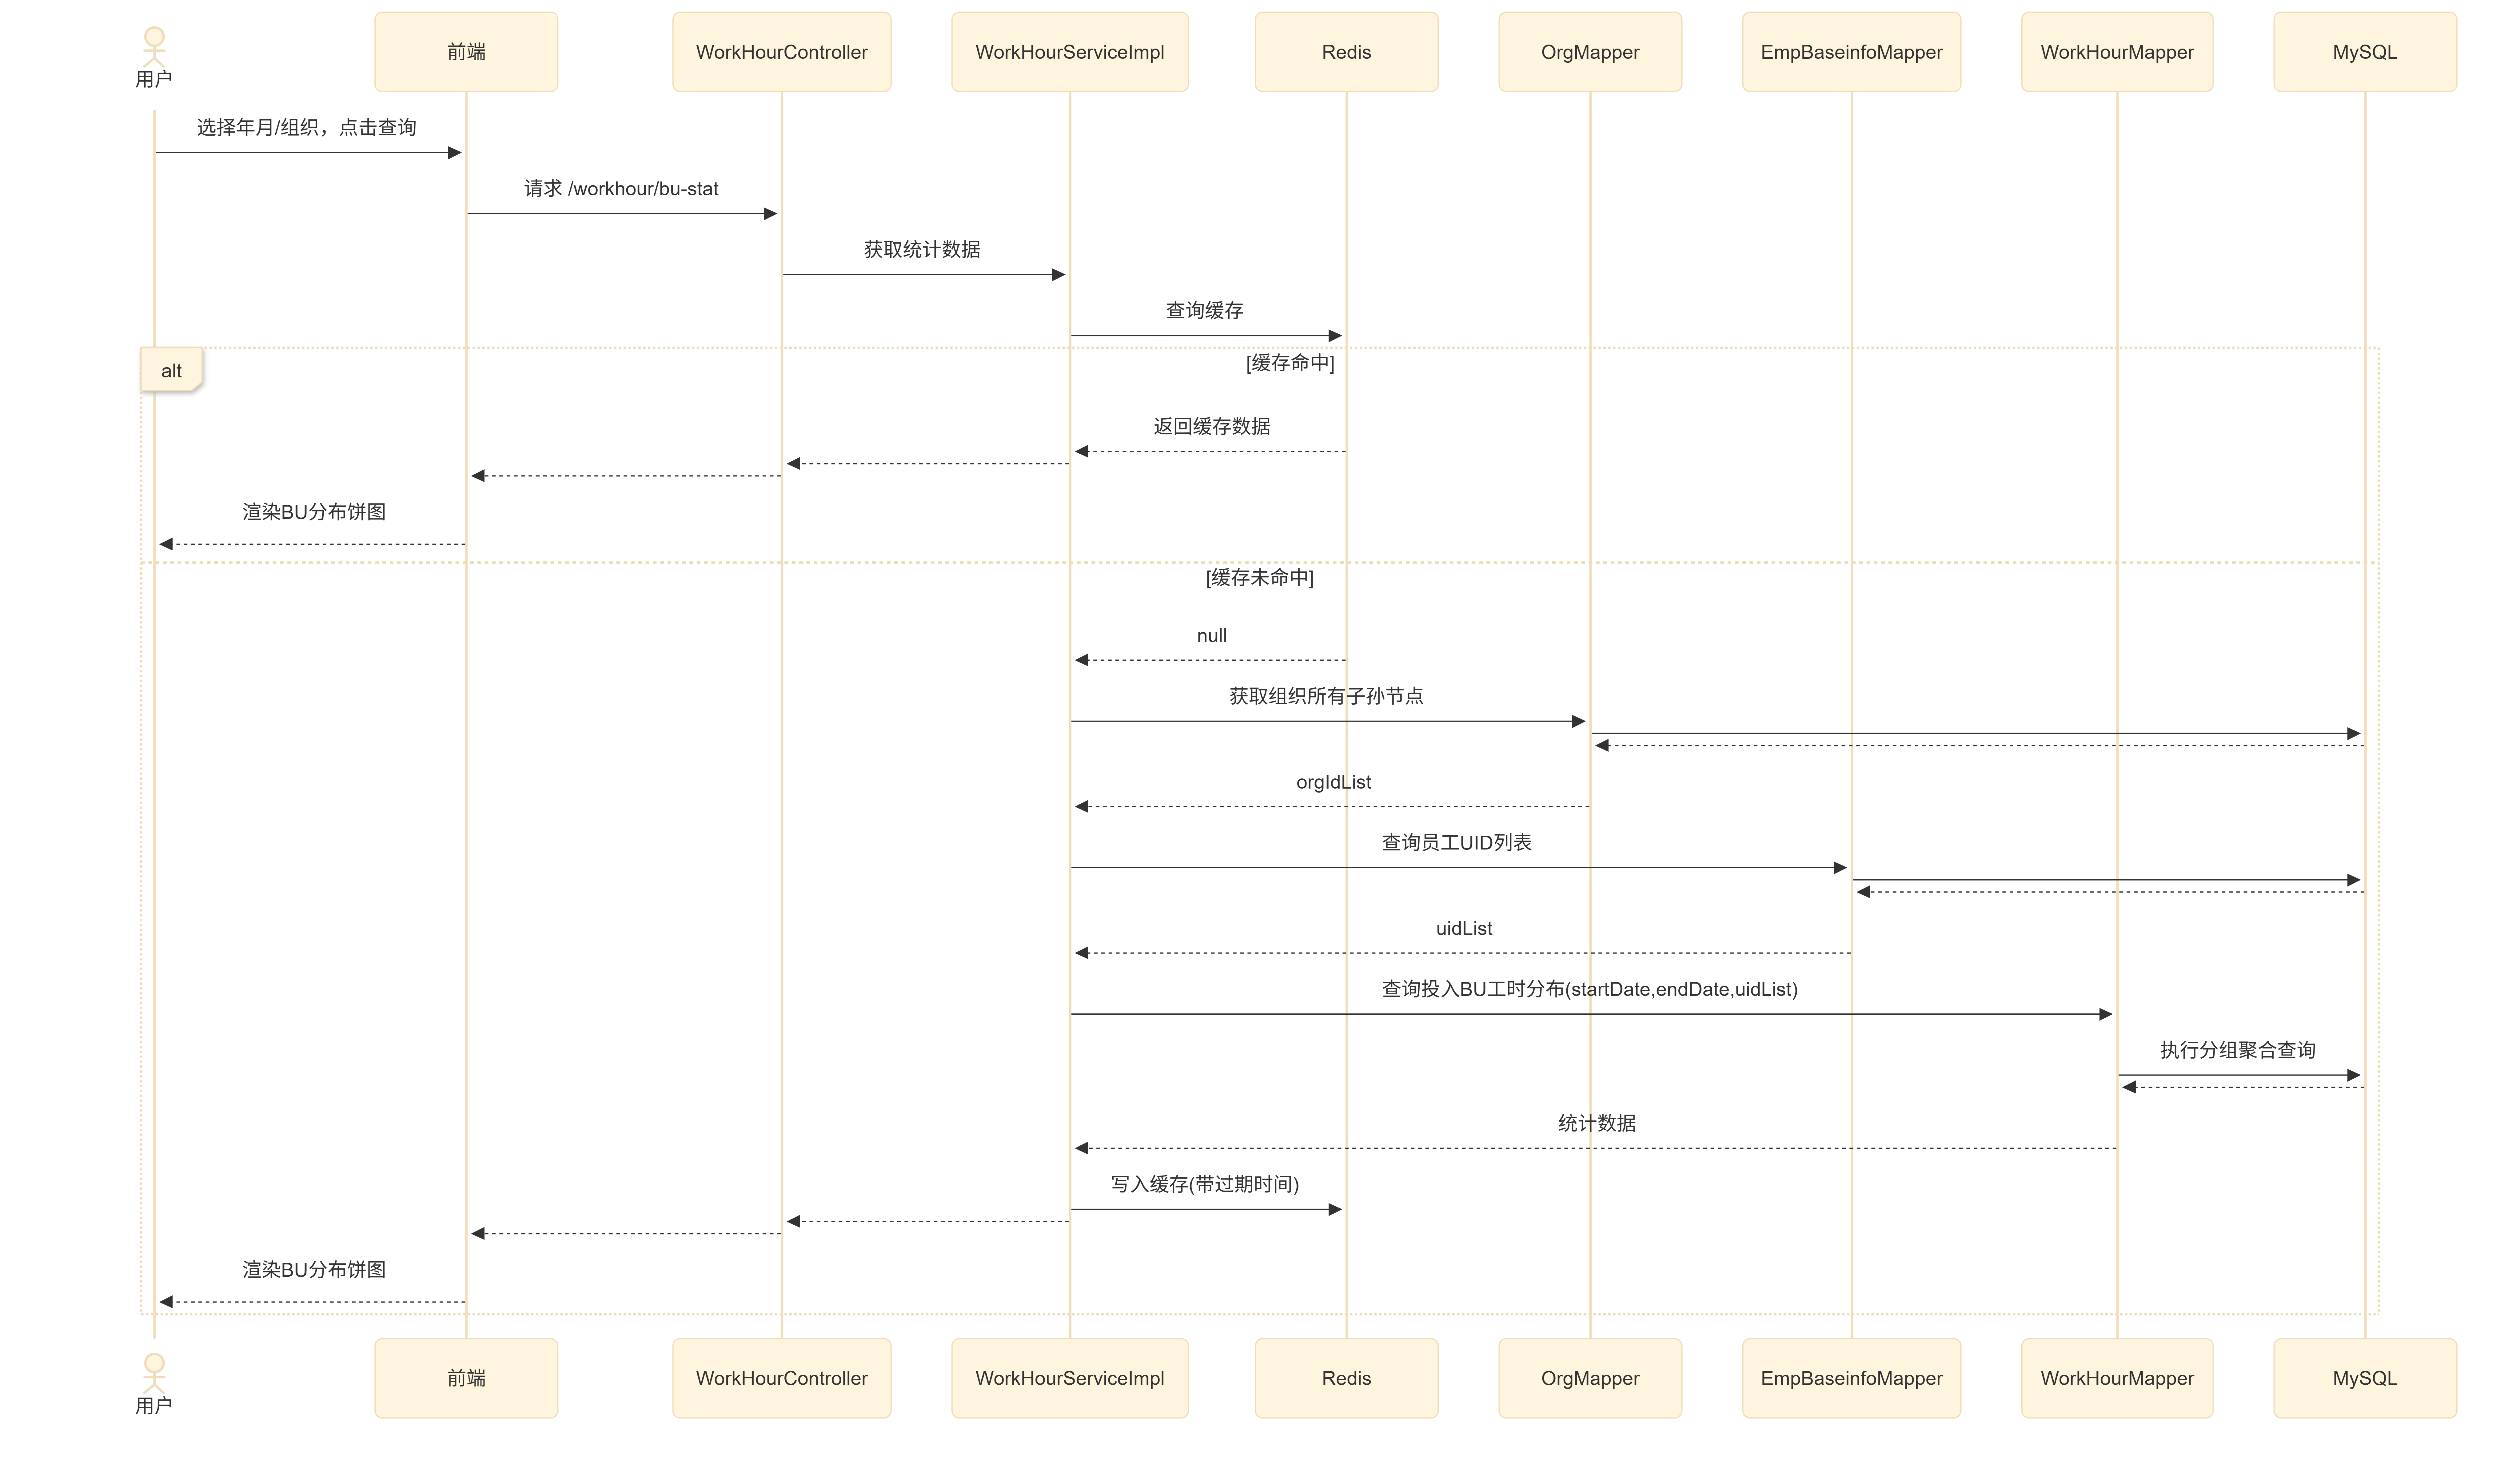
\includegraphics[width=1.0\linewidth]{imgs/Seq/BU工时饼图时序图.png}
	\caption{BU工时饼图时序图}
	\label{fig:seq-bu-hour-distribution}
\end{figure}
用户在前端的下拉框中选择查询的年月和组织节点后，点击查询按钮发起请求。后端请求处理层接收到请求后，首先对参数进行非空和有效性校验，校验通过后进入业务层，首先查询Redis中是否存在对应的图表缓存数据，若命中则直接返回，以此降低到达数据库的请求数量。若缓存未命中，系统首先调用 OrgMapper 递归获取目标组织及其所有子节点的 ID 集合，随后通过 EmployeeMapper 查询出这些节点下所有员工的 UID 列表。同时，针对前端传递的年月参数，考虑到数据库工时表记录的日期精确到天，为避免在 SQL 语句中使用日期格式化函数（如 DATE\_FORMAT）匹配从而引发索引失效问题，业务层会预先将年月参数转换为该月的起止时间范围（即月初第一天至月末最后一天）。接着，将时间参数和 UID 列表传入 WorkHourMapper，调用接口对数据库执行分组聚合查询，计算出各个BU的工时分布情况。最后，系统将该计算结果写入 Redis 并设置过期时间，过期策略是当月数据一小时，其余时间24小时，将数据封装后返回给前端，利用Echarts组件来渲染分布饼图。

用户如果想知道某个BU的工时详情，可以点击对应模块，其核心时序如图\ref{fig:seq-bu-hour-detail}所示。
\begin{figure}[htbp]
	\centering
	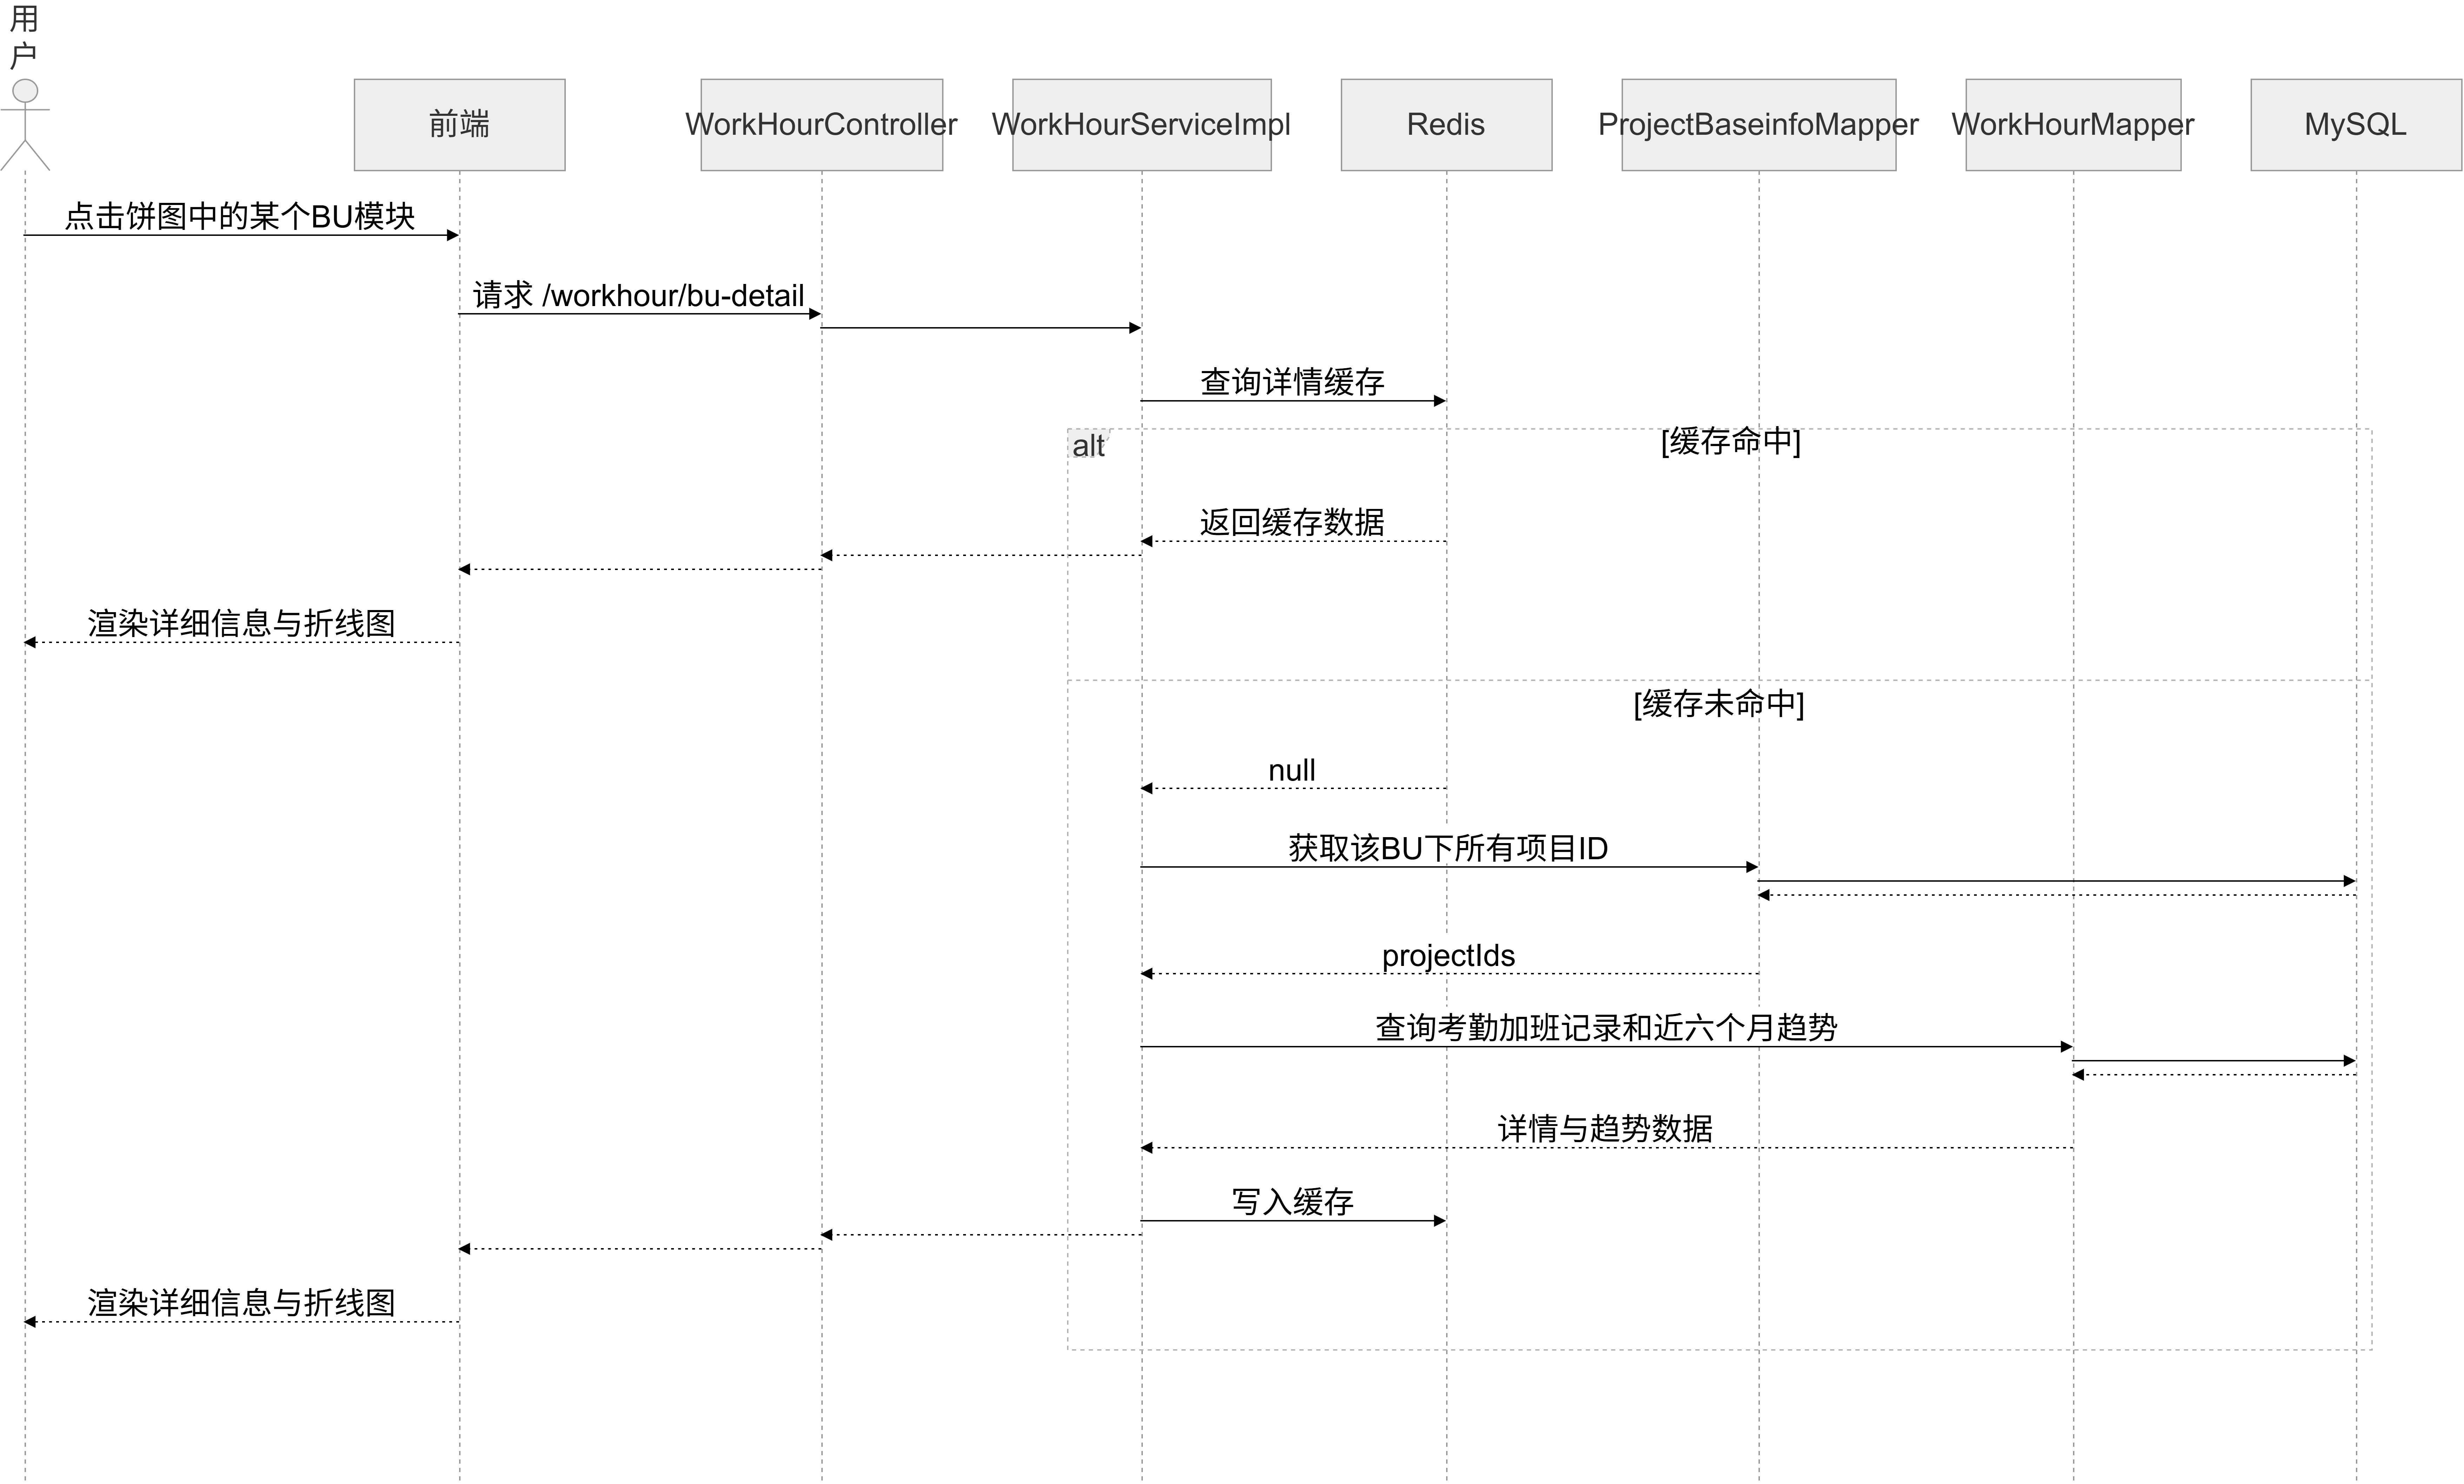
\includegraphics[width=1.0\linewidth]{imgs/Seq/BU详情时序图.png}
	\caption{BU详情时序图}
	\label{fig:seq-bu-hour-detail}
\end{figure}
前端会发起对该 BU 的详情查询请求。后端同样优先进行缓存校验。若缓存未命中，系统首先通过 ProjectMapper 查询出该 BU 下挂载的所有项目 ID 列表。随后，依据项目 ID 调用 WorkHourMapper 查询这些项目的加班工时数和近六个月的工时变化趋势。在将详情数据回写至 Redis时，系统对过期时间进行了抖动处理，以防止大量缓存同时失效引发缓存雪崩问题。数据返回前端后，渲染生成具体的基础信息面板与工时趋势折线图。

\subsection{项目基本信息管理}
项目基本信息维护是玄武平台数字化项目管理部分的一部分。通过该模块，项目经理（SPM）能够对项目的基本信息、里程碑节点及近期交付计划进行统一维护。整个模块的操作主要可划分为基础数据维护与交付节点的高频更新两大维度。

项目基本信息管理类图如图\ref{fig:class-project-baseinfo}所示。
\begin{figure}[htbp]
	\centering
	
\includegraphics[width=1.0\linewidth]{imgs/class/项目基本信息管理类图.png}
	\caption{项目基本信息管理类图}
	\label{fig:class-project-baseinfo}
\end{figure}
在实际开发中，我在 TbProjectBaseinfoController 中定义所有的HTTP接口。对于数据查询操作，使用封装好的 ProjectQueryRequest 参数查询类来接收前端传递的参数，这个类是基类 QueryRequest 的子类，核心的业务逻辑由 TbProjectBaseinfoServiceImpl 承担。内部包含分页查询、新增项目、更新项目、查看更改历史等方法，TbProjectBaseinfoMapper 和 TbProjectBaseinfoHistoryMapper 分别用来与项目基本信息表、项目历史信息表和项目交付历史表进行交互。

其核心业务流转如图\ref{fig:seq-project-baseinfo}所示。
\begin{figure}[htbp]
	\centering
	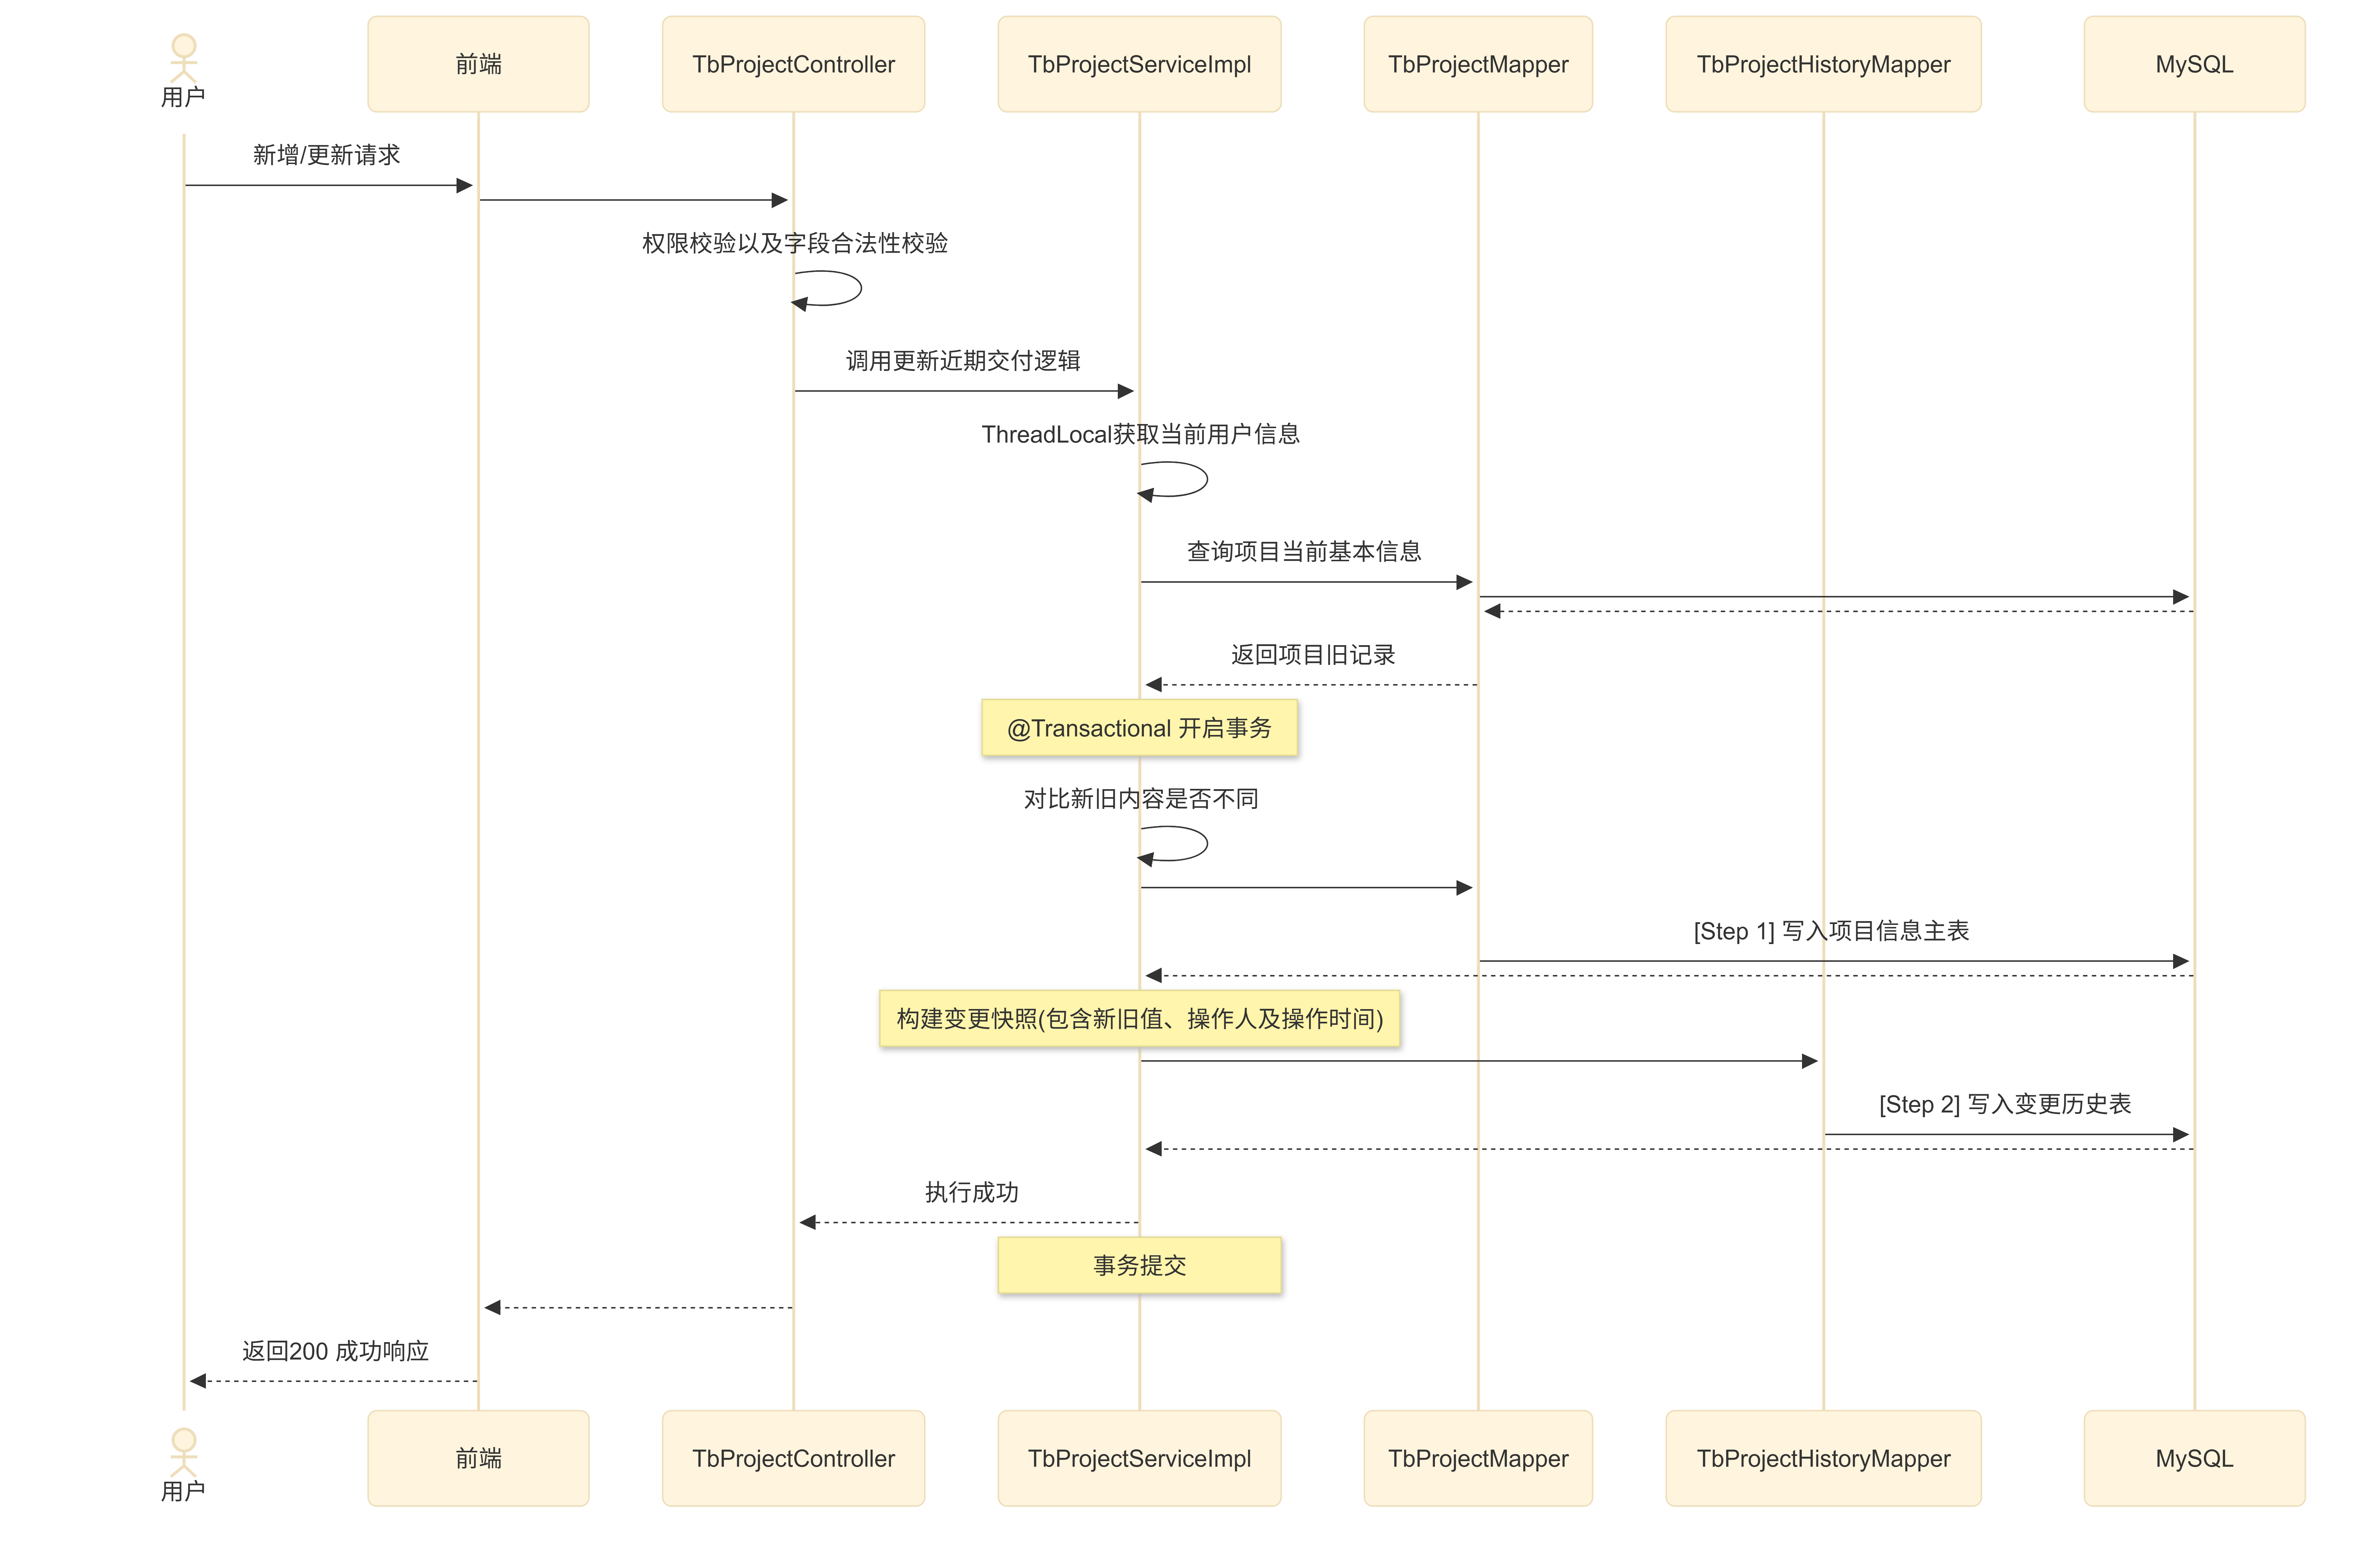
\includegraphics[width=1.0\linewidth]{imgs/Seq/项目信息管理时序图.png}
	\caption{项目信息管理时序图}
	\label{fig:seq-project-baseinfo}
\end{figure}
针对项目基本信息的“新增与更新”流程，系统在后端实现上重点保障了数据的安全性与可追溯性。我们在 TbProjectBaseinfoController 的新增和更新方法上加上了 @RequiresPermissions 注解，前端发起的 HTTP 请求会先经过请求处理层的 JWT 校验，通过后 Shiro 框架会拦截加了注解的方法，在方法执行前先查询预热到缓存的权限数据，如果没有就去数据库查询，检查当前用户是否有对应权限，并利用 \texttt{@Valid} 完成参数的合法性校验。进入业务层后，系统采用“主表+历史表”的双写策略：首先将最新的项目信息更新至MySQL主表；随后，通过构建当前操作的完整数据快照（涵盖新旧值、操作人及操作类型），并写入项目信息快照表。这种快照机制便于后续的项目审计与数据回滚操作。在执行更新操作后，批量清除 Redis 中关联的失效缓存，这样前端在下次查询时能够加载数据库中最新数据。但是由于部分字段比如"近期交付阀点"和"近期阀点日期"修改比较频繁，可能导致快照表的体积变得太大，因此针对这部分的修改历史保存到交付历史变更表中。由于修改了多张表，需要在方法上加上 @Transactional 注解，将多表更新操作限制在单一事务中，以确保原子性和一致性。需要注意的是，在实际开发中，并不是在方法上加注解就可以高枕无忧了，事务包裹的范围应该尽可能小，否则可能会导致长事务的出现，很容易耗尽连接池导致数据库崩溃，同时长期持有的锁会引发大范围阻塞，并因阻碍日志清理而拖垮数据库性能。此外还要考虑注解失效的情景，避免在开发中犯这类错误。

\subsection{缺陷管理}
企业软件项目在研发过程中不可避免地会出现Bug，由于企业实际开发过程中同时使用了多套缺陷跟踪平台，包括Trinity、Jira 和 Bugclose，各平台的缺陷字段各不相同，缺陷管理模块需要对这些缺陷进行统一管理，聚合统计。通过数据汇聚与指标计算，为项目质量人员提供多维度的缺陷质量看板。

缺陷管理类图如图\ref{fig:class-bug}所示。
\begin{figure}[htbp]
	\centering
	
\includegraphics[width=1.0\linewidth]{imgs/class/缺陷管理类图.png}
	\caption{缺陷管理类图}
	\label{fig:class-bug}
\end{figure}
在这个部分定义了 BugQueryRequest 查询类，作为 QueryRequest 的子类，内部设置了自定义的条件过滤器集合，便于对多个字段进行多种条件筛选，业务处理层是该模块的计算核心。BugServiceImpl 注入了 BugMapper 来执行缺陷表的查询操作。BugServiceImpl 还注入了 ProjectClusterService，在处理“项目聚类统计汇总”这一业务时，能调用其中的方法来获取所有聚类名称或者根据聚类名称查询该聚类下的所有挂载项目清单。

（1）项目聚类缺陷统计

缺陷管理部分主要包括缺陷数据的分页查询以及项目聚类缺陷统计，其中，项目聚类缺陷统计的业务流程如图\ref{fig:seq-bug-cluster}所示。
\begin{figure}[!htbp]
	\centering
	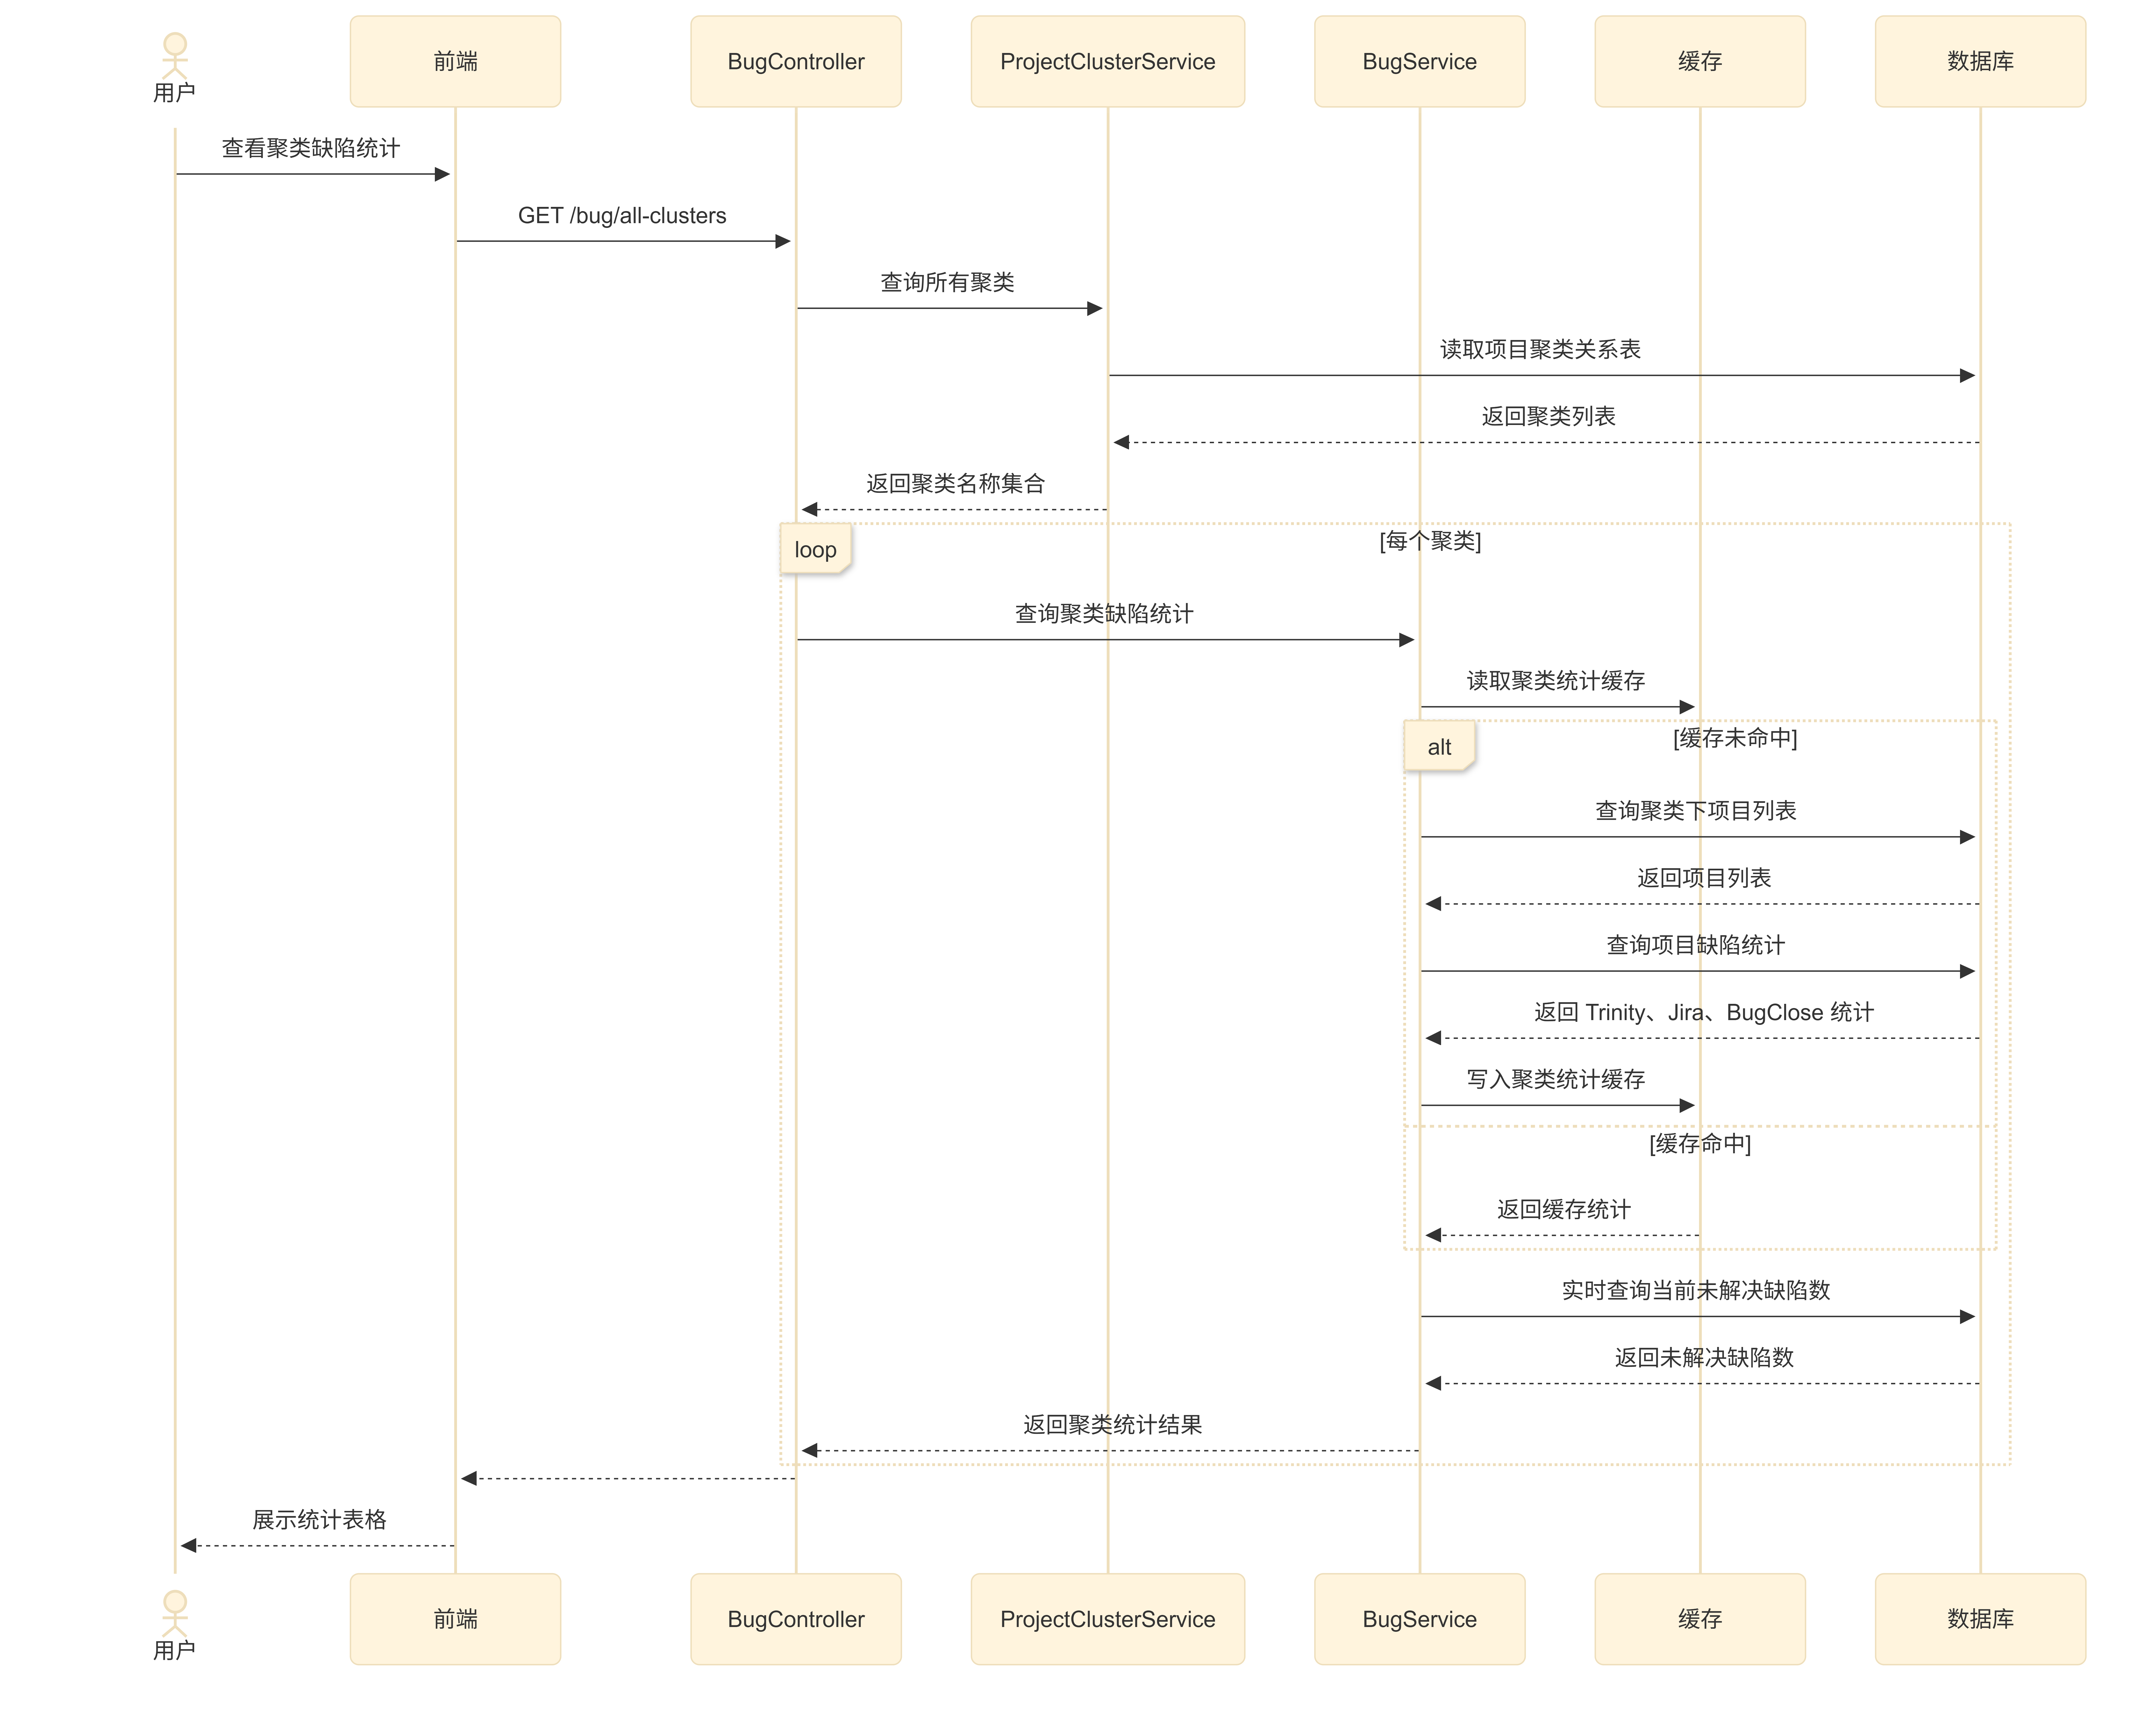
\includegraphics[width=1.0\linewidth]{imgs/Seq/项目聚类缺陷统计时序图.png}
	\caption{项目聚类缺陷统计时序图}
	\label{fig:seq-bug-cluster}
\end{figure}
项目聚类缺陷统计主要用于对多个项目组成的聚类进行缺陷数据汇总分析。系统首先从项目聚类关系表中获取全部聚类名称，并根据聚类名称查询其包含的项目列表。随后，系统以项目为基本统计单元，分别从 Trinity 缺陷表、Jira 缺陷表和 BugClose 缺陷表中提取缺陷数据，并计算当前未解决缺陷数、新增缺陷数、解决缺陷数、超期未解决缺陷数以及关闭率等指标。最后以表格的形式展示给用户，对于一些关闭率低的项目聚类，还设置了定时任务发送飞书预警消息来提醒。

考虑到聚类缺陷统计涉及多个数据表，查询成本较高，系统在设计中引入缓存机制。对于昨日新增、昨日解决、总缺陷数、关闭数以及聚类级历史统计等变化频率较低的数据，系统使用缓存保存统计结果；对于当前未解决缺陷数等实时性要求较高的数据，则在接口调用时进行实时计算，并与缓存结果合并后返回。该设计在保证统计结果实时性的同时，降低了数据库访问压力，提高了聚类缺陷看板的响应效率。

（2）缺陷数据深分页优化

系统的缺陷数据来自于三个外部平台（Trinity,Jira,BugClose），分别存储至数据库的三张同步表（"tb\_sync\_bug"、"tb\_sync\_jira"、"tb\_sync\_bugclose"），然后在前端进行分页查询。由于缺陷数据表的体积非常大，无论是进行分页查询还是excel导出时都会出现较大的延迟。excel导出由于内存里放不下这么多数据，可以参考外部排序的思想，利用游标来分批获取数据并写入Excel。对于深分页，出现这个问题的原因是因为对于 LIMIT offset, N，MySQL 并非直接跳到 offset 处，而是必须从头扫描 offset + N 条记录。如果查询依赖二级索引且不满足覆盖索引，这意味着 MySQL 需要对前 offset 条记录执行毫无意义的回表查询（产生海量的随机 I/O），最后再将这些辛苦查出的数据丢弃。即便优化器最终因代价过高退化为全表扫描，顺序扫描百万行的成本依然巨大。对于分页查询来说，我们可以通过延迟关联将 LIMIT 操作转移到主键索引树上，减少回表次数，再通过INNER JOIN将子查询结果集成到主查询中。
\begin{figure}[htbp]
	\centering
	\noindent % 消除首行缩进，确保左侧完全对齐
	\begin{minipage}[t]{0.42\textwidth}
		\textbf{优化前（传统单表分页）}
		\begin{lstlisting}[language=SQL, frame=single, basicstyle=\ttfamily\small, breaklines=true, tabsize=4]
			SELECT * FROM tb_sync_bug
			WHERE severity = 'A'
			ORDER BY created_date DESC
			LIMIT 100000, 20
		\end{lstlisting}
	\end{minipage}
	\hfill
	\begin{minipage}[t]{0.54\textwidth}
		\textbf{优化后（延迟关联分页）}
		\begin{lstlisting}[language=SQL, frame=single, basicstyle=\ttfamily\small, breaklines=true, tabsize=4]
			SELECT b.* FROM tb_sync_bug b
			INNER JOIN (
			SELECT id, created_date FROM tb_sync_bug
			WHERE severity = 'A'
			ORDER BY created_date DESC, id ASC
			LIMIT 100000, 20
			) page_ids ON page_ids.id = b.id
			ORDER BY page_ids.created_date DESC, page_ids.id ASC
		\end{lstlisting}
	\end{minipage}
	\caption{深分页优化前后 SQL 语句横向对比}
	\label{fig:sql-optimization-compare}
\end{figure}

\subsection{重大问题管理}
% 模块功能设计
重大问题管理模块面向项目执行过程中影响范围较大、处理周期较长或需要跨部门协调的问题，大致可分为问题登记、问题处理和问题关闭三个阶段。具体流程如图\ref{fig:serious-problem-process}所示。
\begin{figure}[htbp]
	\centering
	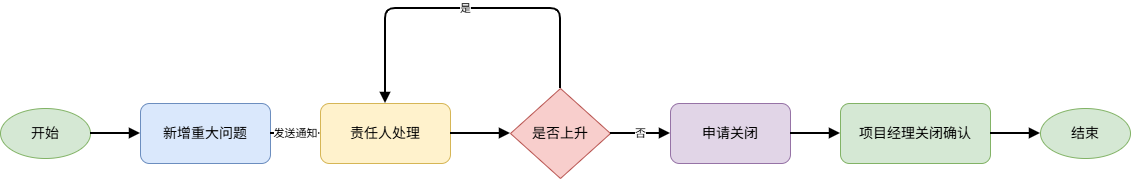
\includegraphics[width=1.0\linewidth]{imgs/Flowchart/重大问题流程图.drawio.png}
	\caption{重大问题流程图}
	\label{fig:serious-problem-process}
\end{figure}

重大问题管理类图如图\ref{fig:class-serious-problem}所示。
\begin{figure}[htbp]
	\centering
	
\includegraphics[width=1.0\linewidth]{imgs/class/重大问题管理类图.png}
	\caption{重大问题管理类图}
	\label{fig:class-serious-problem}
\end{figure}
这部分功能主要围绕实体类 TbProjectSeriousProblem 展开，在控制层提供了分页查询，新增/更新，导出excel以及发送飞书提醒消息的功能，到了业务层，可以通过员工服务ITbEmpBaseinfoService的相关接口补全关联项目与干系人的元数据；其次，发送飞书消息时需要根据重大问题是否上升处理来调整接收人列表，通过调用OrgService的fetchOrgLeaderByOrganCode() 方法在组织树中向上递归溯源，精准定位并提取根因部门的组织负责人信息，最后将组织好的上下文交给IFeishuService，利用其 sendTemplateCard() 方法渲染为飞书消息卡片并发送。

重大问题管理的核心业务流程如图\ref{fig:seq-serious-problem}所示。用户进入列表页面后，系统首先根据当前登录用户的身份判断其权限，查询并展示其可见的问题记录。用户可通过顶部筛选栏按多维度条件进行检索，也可点击"新增"按钮创建新的重大问题。
\begin{figure}[!htbp]
	\centering
	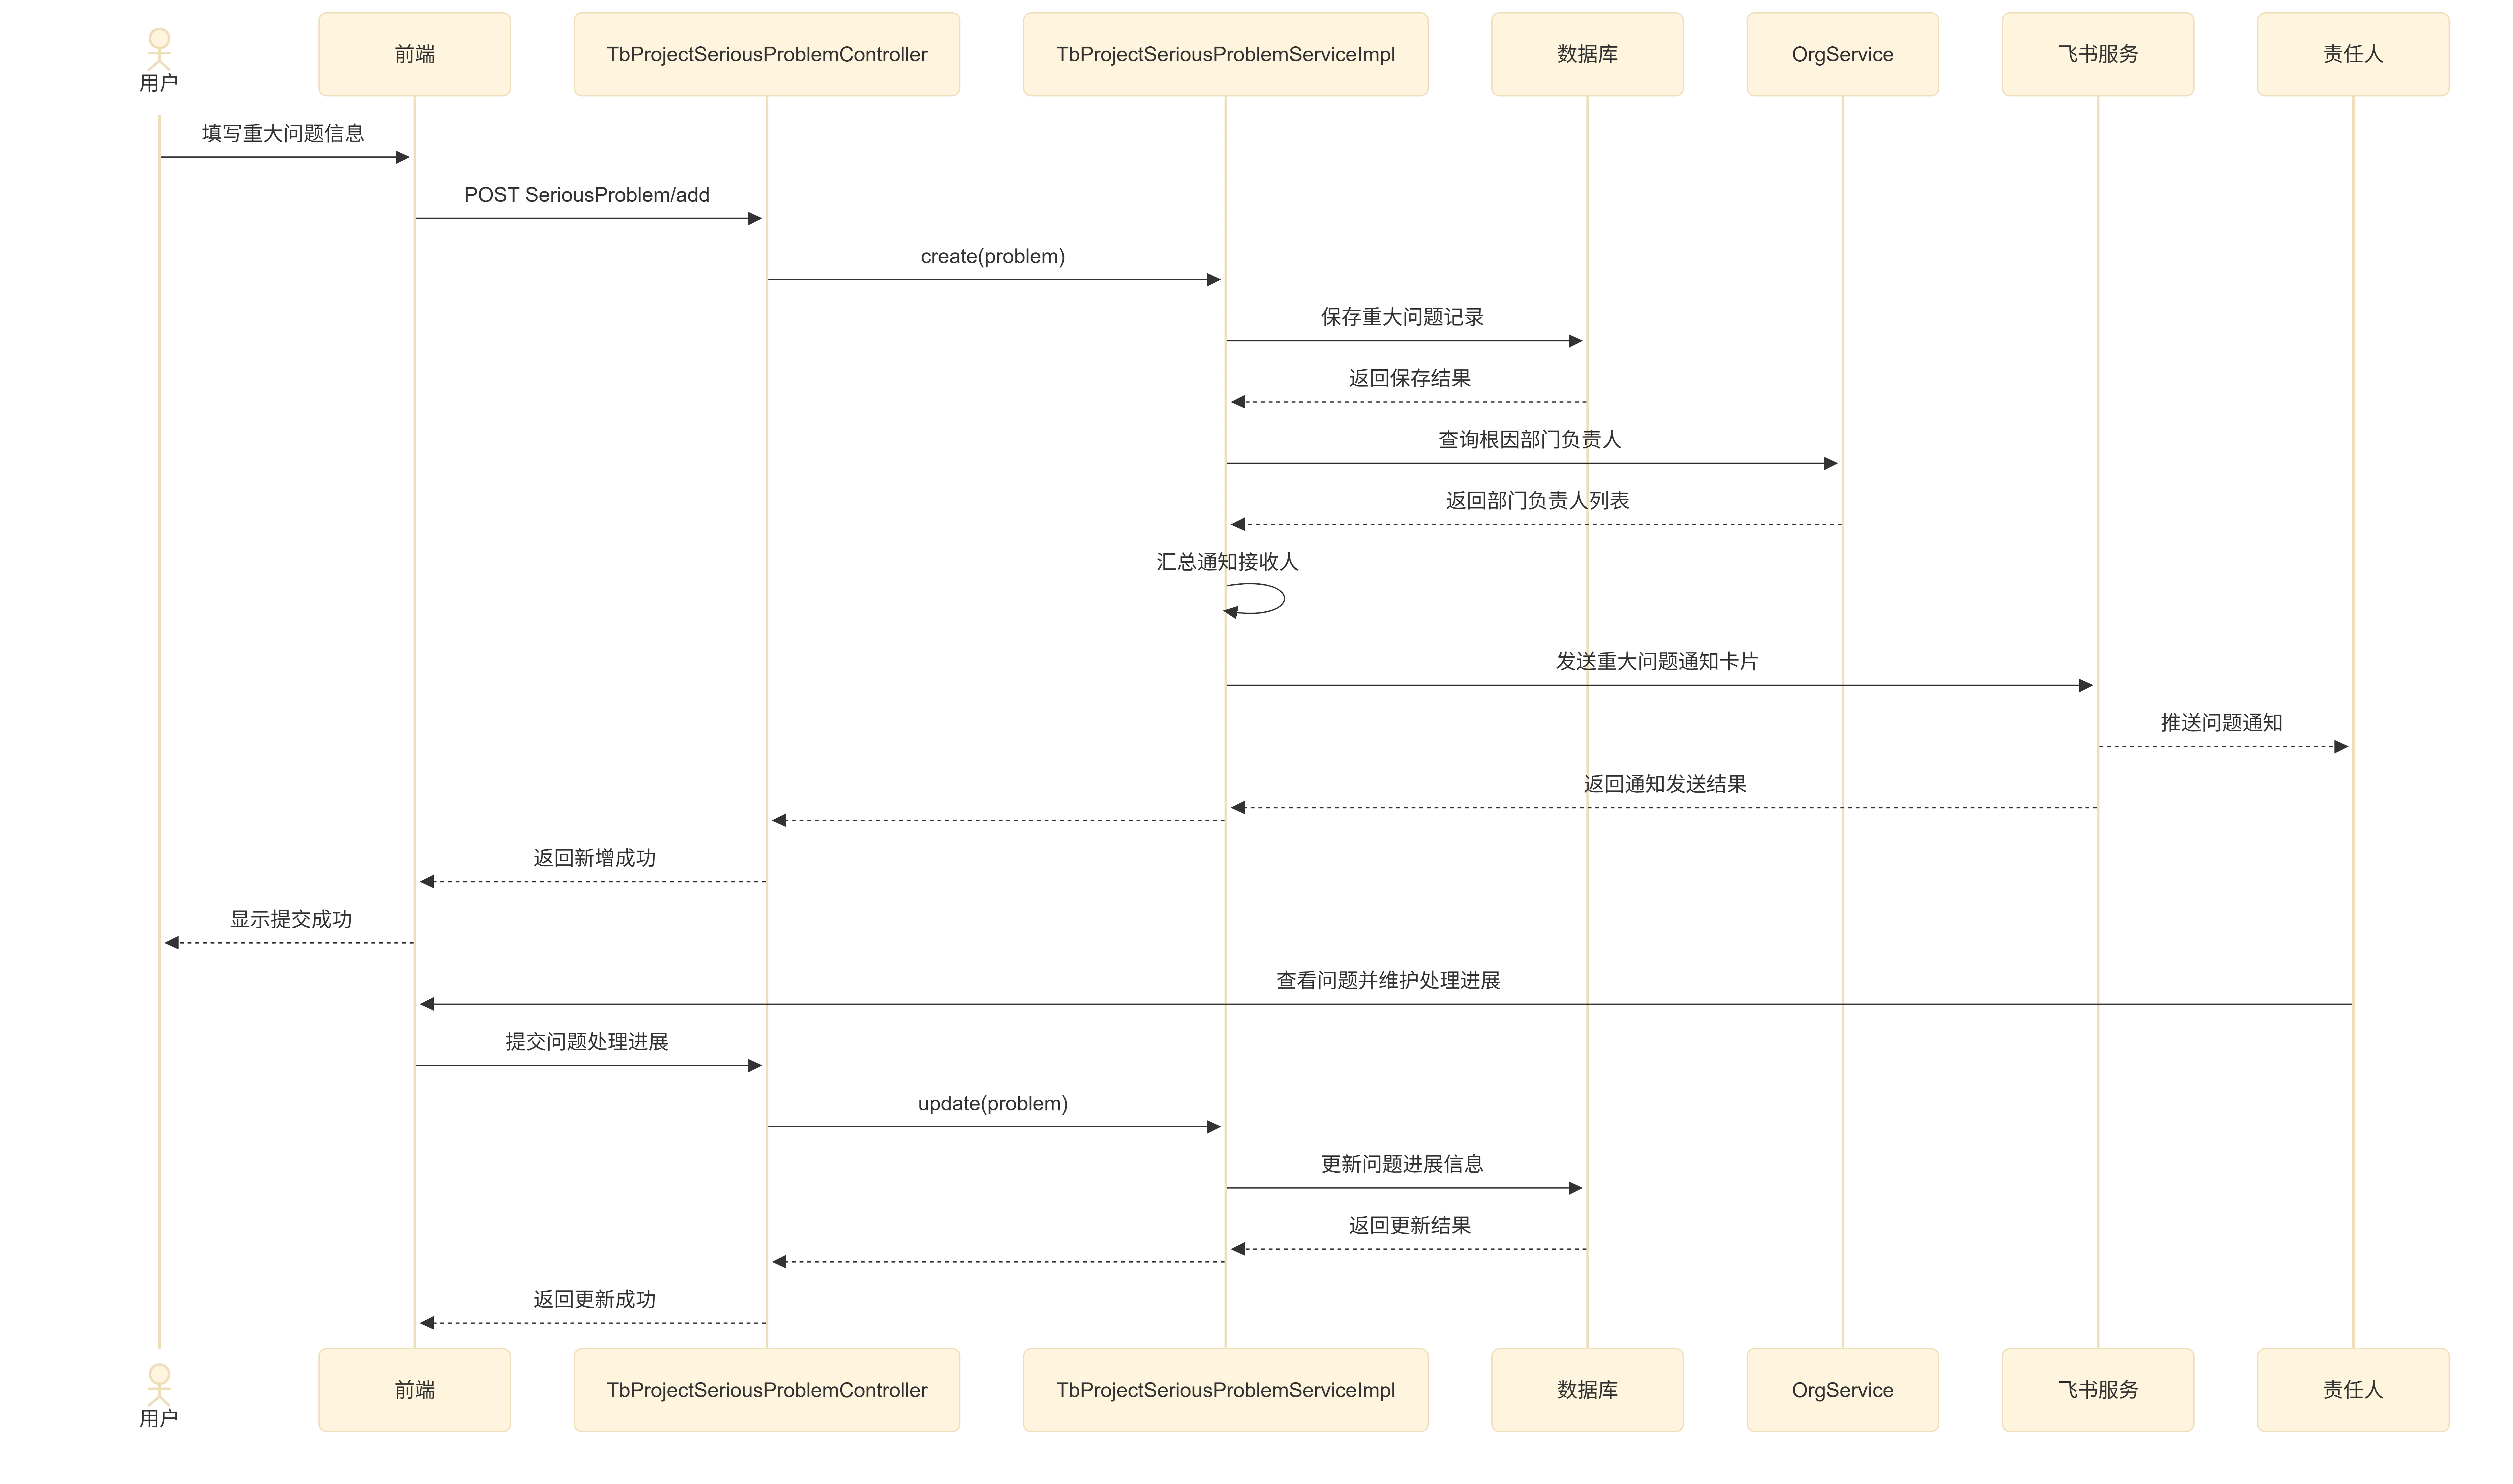
\includegraphics[width=1.0\linewidth]{imgs/Seq/重大问题时序图.png}
	\caption{重大问题时序图}
	\label{fig:seq-serious-problem}
\end{figure}

在问题登记阶段，用户填写重大问题的基础信息和首问闭环责任人。系统保存记录后，根据问题涉及的责任人生成通知内容，并通过飞书消息推送给相关人员，使问题能够及时进入处理环节。在问题处理阶段，由责任人来填写问题的技术原因和解决方案；当问题需要更高层级协调时，可将问题标记为“需要上升”，并指定上升责任人，由其介入协调资源后继续推进问题处理。当问题需要关闭时，用户需要补充实际解决日期、最终责任人、责任分类、技术原因、技术解决方案等信息。系统根据计划解决日期和实际解决日期自动判断问题状态：实际解决日期不晚于计划解决日期时，问题状态为按时关闭；实际解决日期晚于计划解决日期时，问题状态为超期关闭；若超过计划解决日期仍未填写实际解决日期，则问题保持超期未关闭状态。通过该设计，模块能够对重大问题从发现、处理、上升到关闭的全过程进行记录和约束。

\section{数据库设计}
为说明系统中各业务数据对象之间的关系，本文首先给出数据库的总体逻辑 ER 图，如图 \ref{fig:er-overall} 所示。该图从业务对象角度抽象出组织、员工、项目、缺陷、重大问题、项目聚类和聚类缺陷快照等核心实体，并描述各实体之间的主要关联关系。后续小节将在此基础上分别说明关键数据表的字段设计。

\subsection{数据库总体设计}
\begin{figure}[htbp]
	\centering
	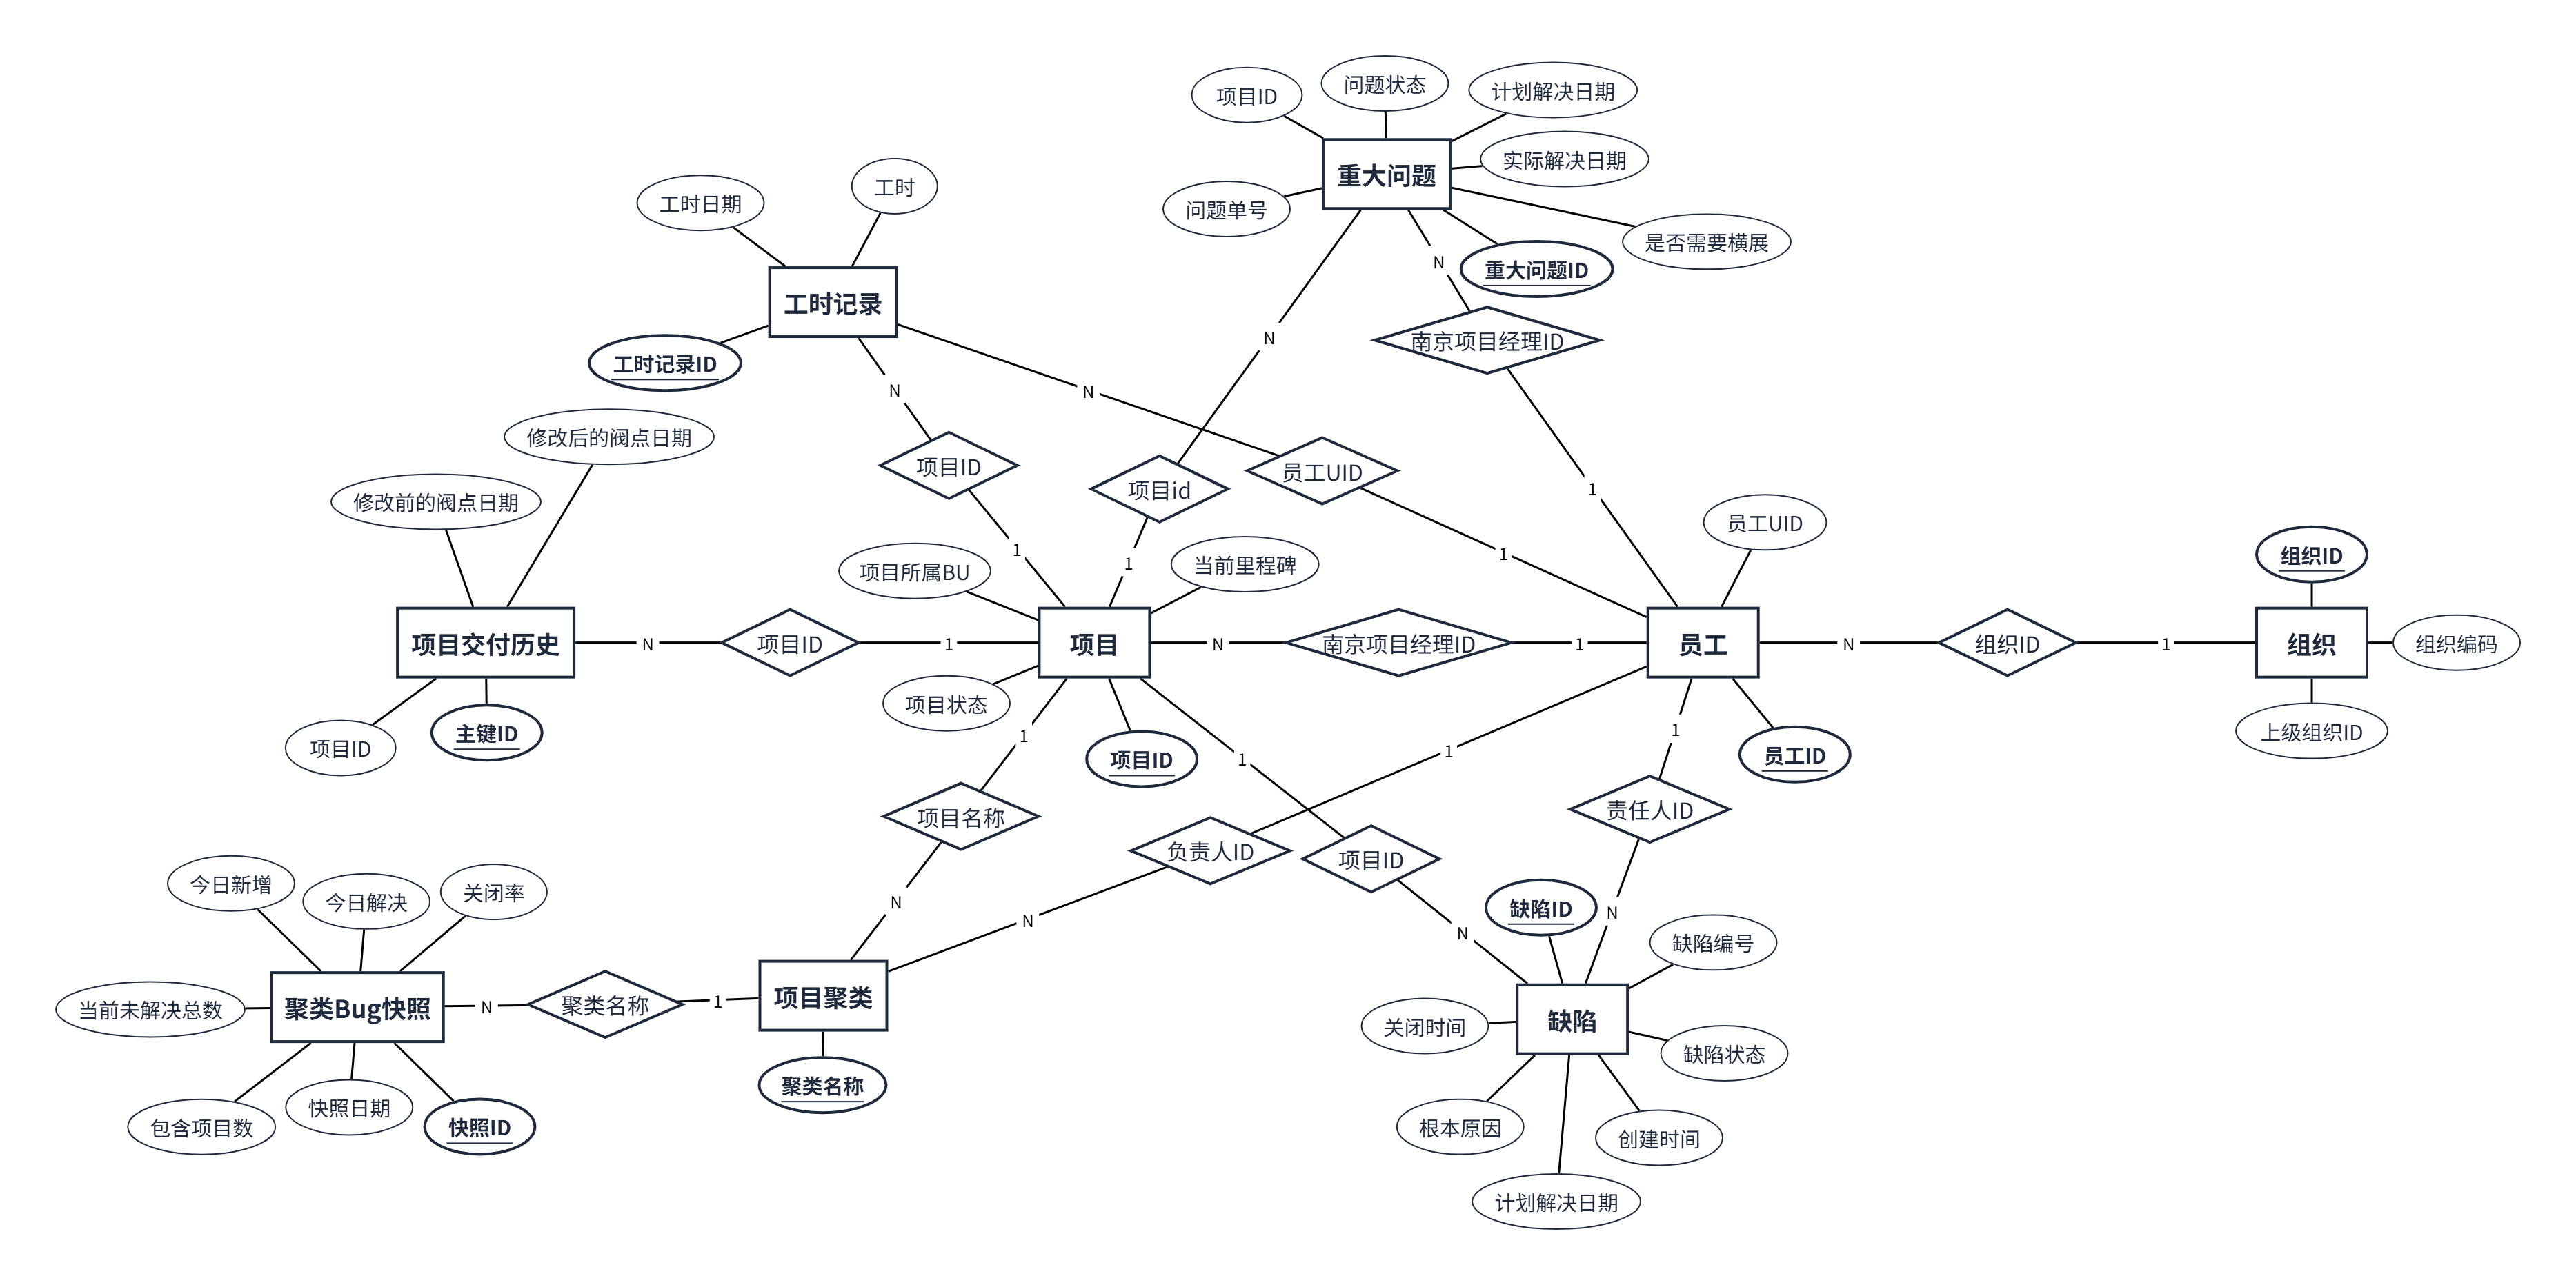
\includegraphics[width=1.0\linewidth]{imgs/ER/er-diagram.png}
	\caption{数据库E-R图}
	\label{fig:er-overall}
\end{figure}
系统数据库以项目为主要业务对象进行组织。项目在系统中既是缺陷统计、工时记录和重大问题管理的归属对象，也是项目聚类分析的基础单元。因此，在总体 ER 图中，项目实体位于业务数据关系的中心位置，并分别与缺陷、重大问题、工时记录、项目交付历史和项目聚类等实体建立联系。

组织和员工实体用于描述系统中的人员基础数据。组织实体记录组织编号、组织编码以及上级组织编号，用于表示企业内部的层级结构；员工实体记录员工编号、员工 UID 以及所属组织。员工与组织之间是一对多关系，即一个组织下可以包含多名员工，而每名员工归属于一个组织。

项目实体记录项目状态、项目所属 BU、南京项目经理、当前里程碑、近期交付阀点及阀点日期等信息。项目与员工之间通过项目经理的id建立关联，一个项目经理可以负责多个项目。项目交付历史实体用于记录项目近期交付的变更情况。该实体与项目实体之间是一对多关系，表示同一项目在执行过程中可能产生多次交付节点调整记录。

缺陷实体用于保存项目缺陷的主要信息。缺陷与项目之间是一对多关系，一个项目可以对应多条缺陷记录；缺陷与员工之间通过责任人建立关联，用于定位缺陷处理人员。

重大问题实体用于记录项目执行过程中需要重点跟踪的问题。重大问题与项目之间是一对多关系，即一个项目可以产生多条重大问题记录。

项目聚类是指将多个相关项目归为一组，以组为单位进行缺陷统计。系统通过聚类名称将若干项目归为同一统计对象，并为聚类配置负责人。项目聚类与项目之间形成一对多关系，一个聚类可以包含多个项目；项目聚类与员工之间通过负责人建立关联，用于表示该聚类统计对象的管理责任人。聚类 Bug 快照与项目聚类之间是一对多关系，同一聚类可以按日期保存多条快照记录，从而支持缺陷趋势分析。

总体来看，该数据库模型以项目为中心，将人员组织、缺陷数据、重大问题、工时记录、交付历史和聚类统计数据连接起来。组织和员工实体提供人员归属关系，项目实体承载项目基础信息，缺陷和重大问题实体记录项目执行过程中的质量问题，项目聚类和聚类 Bug 快照实体则面向跨项目统计分析。由于部分业务数据来源于外部同步表，实际物理表中并非所有关系都采用数据库外键约束，图中的关系主要用于描述系统业务对象之间的逻辑关联。

\subsection{数据表结构设计}
\begin{enumerate}[label=(\arabic*)]	
	\item BU工时统计主要用于分析各个组织部门在业务单元的工时投入情况，涉及的实体包括组织树（\texttt{tb\_org\_tree}）、员工基础信息（\texttt{tb\_emp\_baseinfo}）、项目列表（\texttt{tb\_project\_\allowbreak baseinfo\_\allowbreak new}）、工时记录（\texttt{tb\_sync\_wh}）和考勤工时（\texttt{tb\_sync\_attend\_hour}），其关系如图\ref{fig:er-org-wh}所示。
	
	\begin{figure}[htbp]
		\centering
		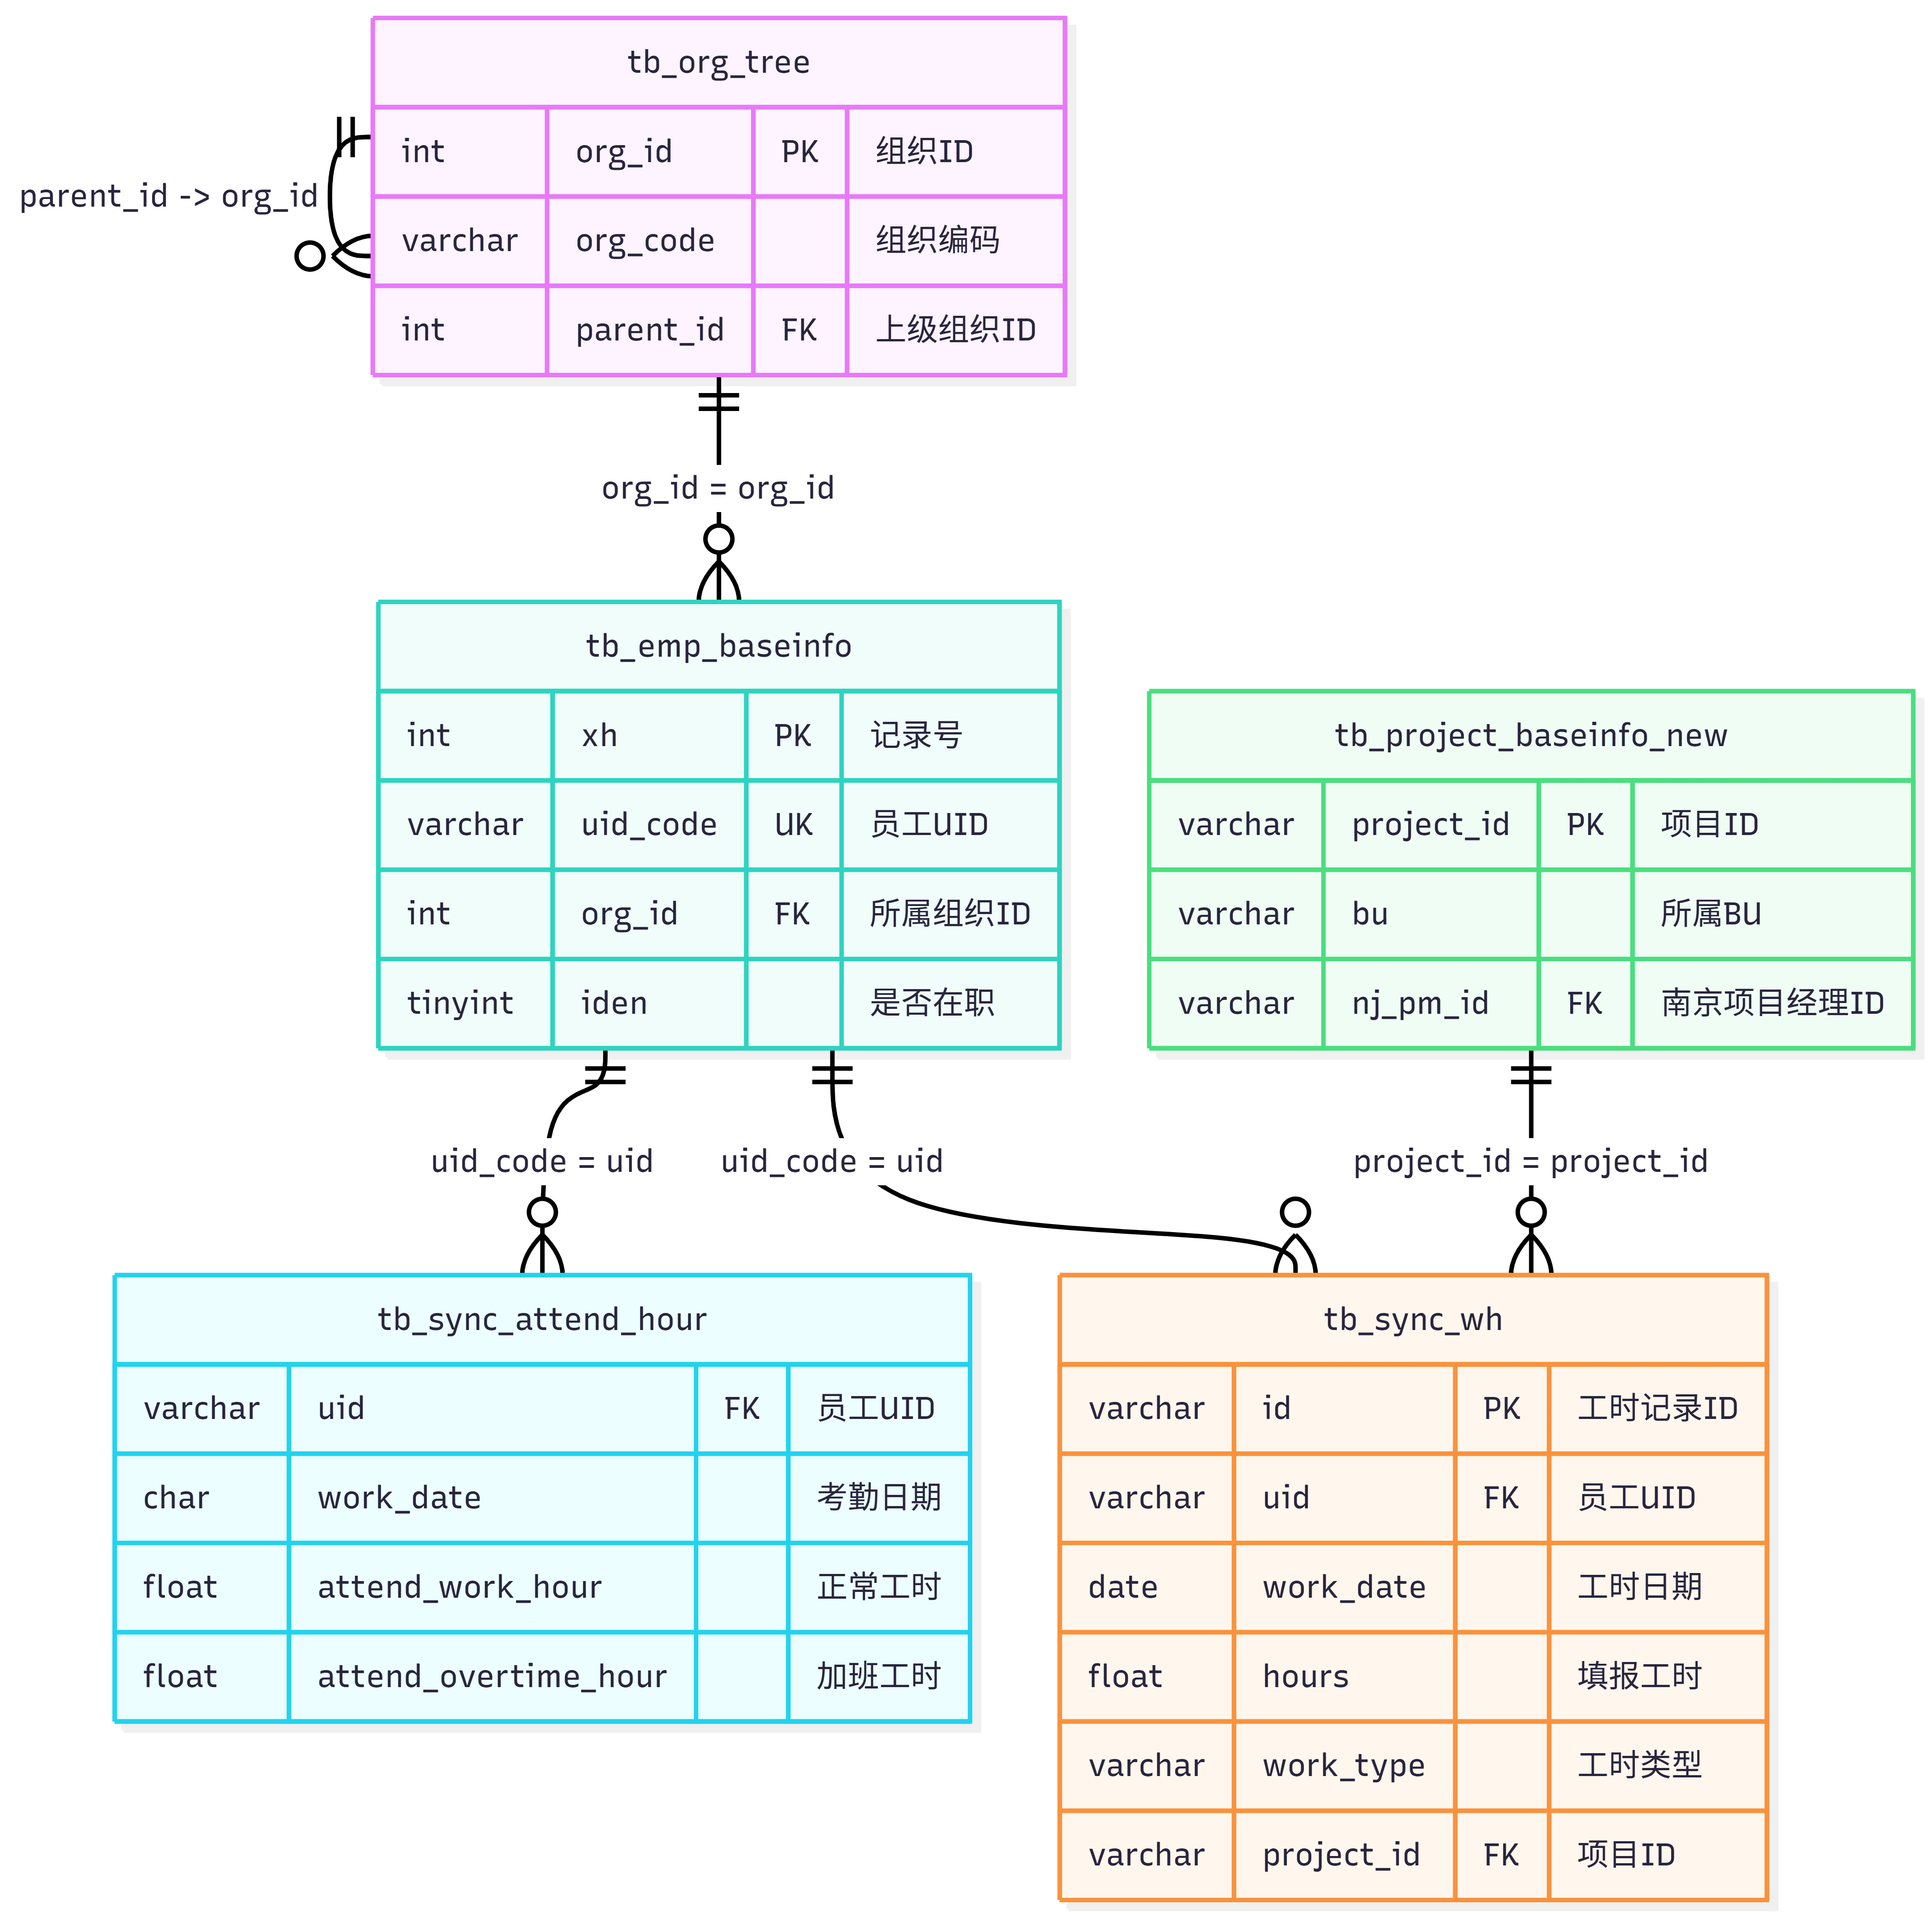
\includegraphics[width=0.7\linewidth]{imgs/ER图-部门投入BU工时分析.png}
		\caption{工时E-R图}
		\label{fig:er-org-wh}
	\end{figure}
	
	在该 E-R 模型中，\verb|tb_org_tree| 用于保存组织树结构，通过 \verb|parent_id| 与 \verb|org_id| 的自关联关系描述组织上下级层级。\verb|tb_emp_baseinfo| 用于保存员工基础信息，其中 \verb|org_id| 表示员工所属组织，\verb|uid_code| 是员工在系统中的唯一标识。工时记录表 \verb|tb_sync_wh| 存储从 Trinity 系统同步而来的员工填报工时数据，通过 \verb|uid| 与员工表中的 \verb|uid_code| 建立逻辑关联，通过 \verb|project_id| 与项目基础信息表中的 \verb|project_id| 建立逻辑关联。考勤工时表 \verb|tb_sync_attend_hour| 保存员工每日考勤工时、加班工时和填写工时等数据，同样通过 \verb|uid| 与员工表关联。
	
	该模型能够支撑 BU 工时趋势分析、BU 加班工时统计和 BU 工时占比分析等功能。系统的接口首先接收年月、组织ID作为参数，根据组织树获取目标部门下的员工范围，然后根据员工范围查询指定时间范围内的工时记录，并结合项目所属 BU 字段完成按 BU 的聚合统计。同时，通过考勤工时表中的加班字段，可以进一步计算某个 BU 的加班投入情况以及近几个月的工时趋势。
	
	\item 项目基本信息管理是项目运营管理模块的基础，其数据模型围绕项目主数据展开，并关联项目交付历史、项目里程碑和项目负责人等信息，涉及的实体包括员工信息、项目基本信息、交付历史（\verb|tb_project_delivery_history|）和里程碑（\verb|tb_project_milestone|），其关系如图\ref{fig:er-project}所示
	
	\begin{figure}[htbp]
		\centering
		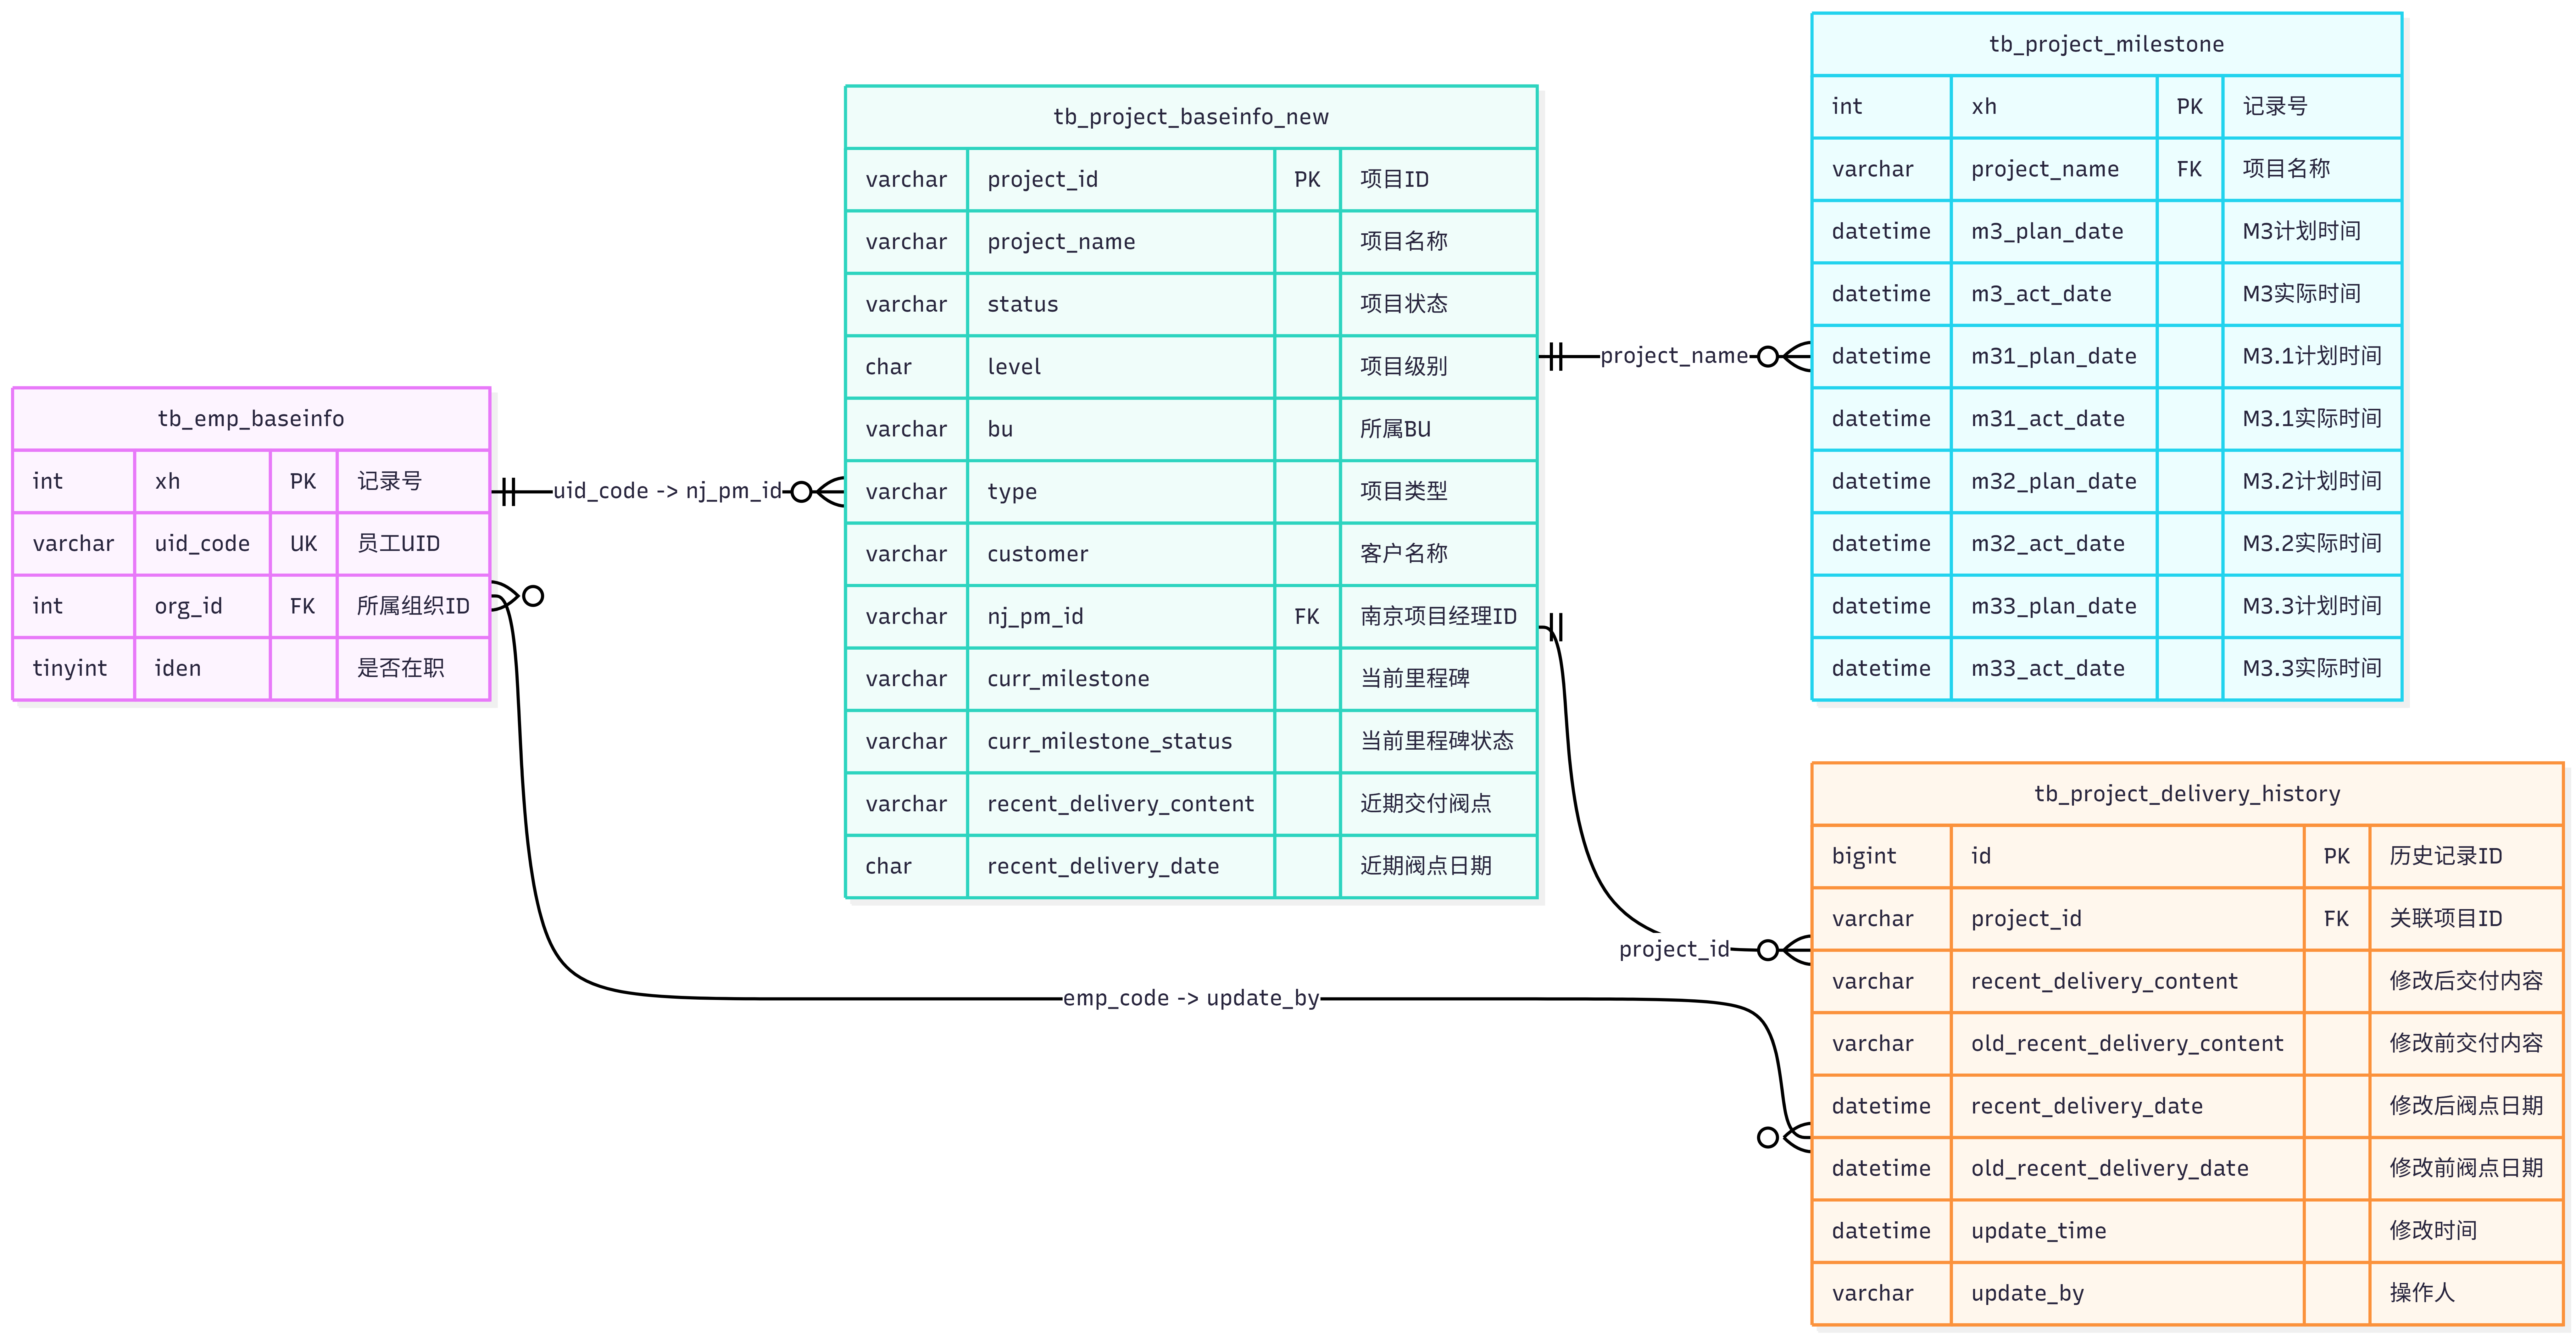
\includegraphics[width=0.7\linewidth]{imgs/ER图-项目代码.png}
		\caption{项目基本信息E-R图}
		\label{fig:er-project}
	\end{figure}
	
	项目基础信息表 \verb|tb_project_baseinfo_new| 是该模型中的核心实体，用于保存项目编号、项目名称、项目状态、项目级别、所属 BU、项目类型、客户名称、南京项目经理、当前里程碑和近期交付阀点等信息。员工基础信息表 \verb|tb_emp_baseinfo| 通过 \verb|uid_code| 与项目表中的 \verb|nj_pm_id| 建立逻辑关联，用于描述项目与南京项目经理之间的责任关系。
	\verb|tb_project_delivery_history| 用于保存项目近期交付内容的修改历史。当项目周报中的近期交付内容或交付日期发生变化时，系统会将修改前后的内容、修改时间以及操作人记录到该表中，从而实现项目交付信息的历史追溯。该表通过 \verb|project_id| 与项目基础信息表关联。\verb|tb_project_milestone| 用于记录项目 M3、M3.1、M3.2、M3.3 等关键阶段的计划时间和实际时间，通过 \verb|project_name| 与项目基础信息表形成逻辑关联。
	通过该 E-R 模型，系统能够支持项目基础信息分页查询、组合筛选、项目信息维护、里程碑维护和周报交付历史追踪等功能。
	
	
	\item 缺陷查询与统计模块需要整合来自 Trinity、Jira 和 BugClose 等多个缺陷平台的数据，并在此基础上支持项目维度和项目聚类维度的缺陷统计分析。其关系如图\ref{fig:er-bug-cluster}所示。
	
	\begin{figure}[htbp]
		\centering
		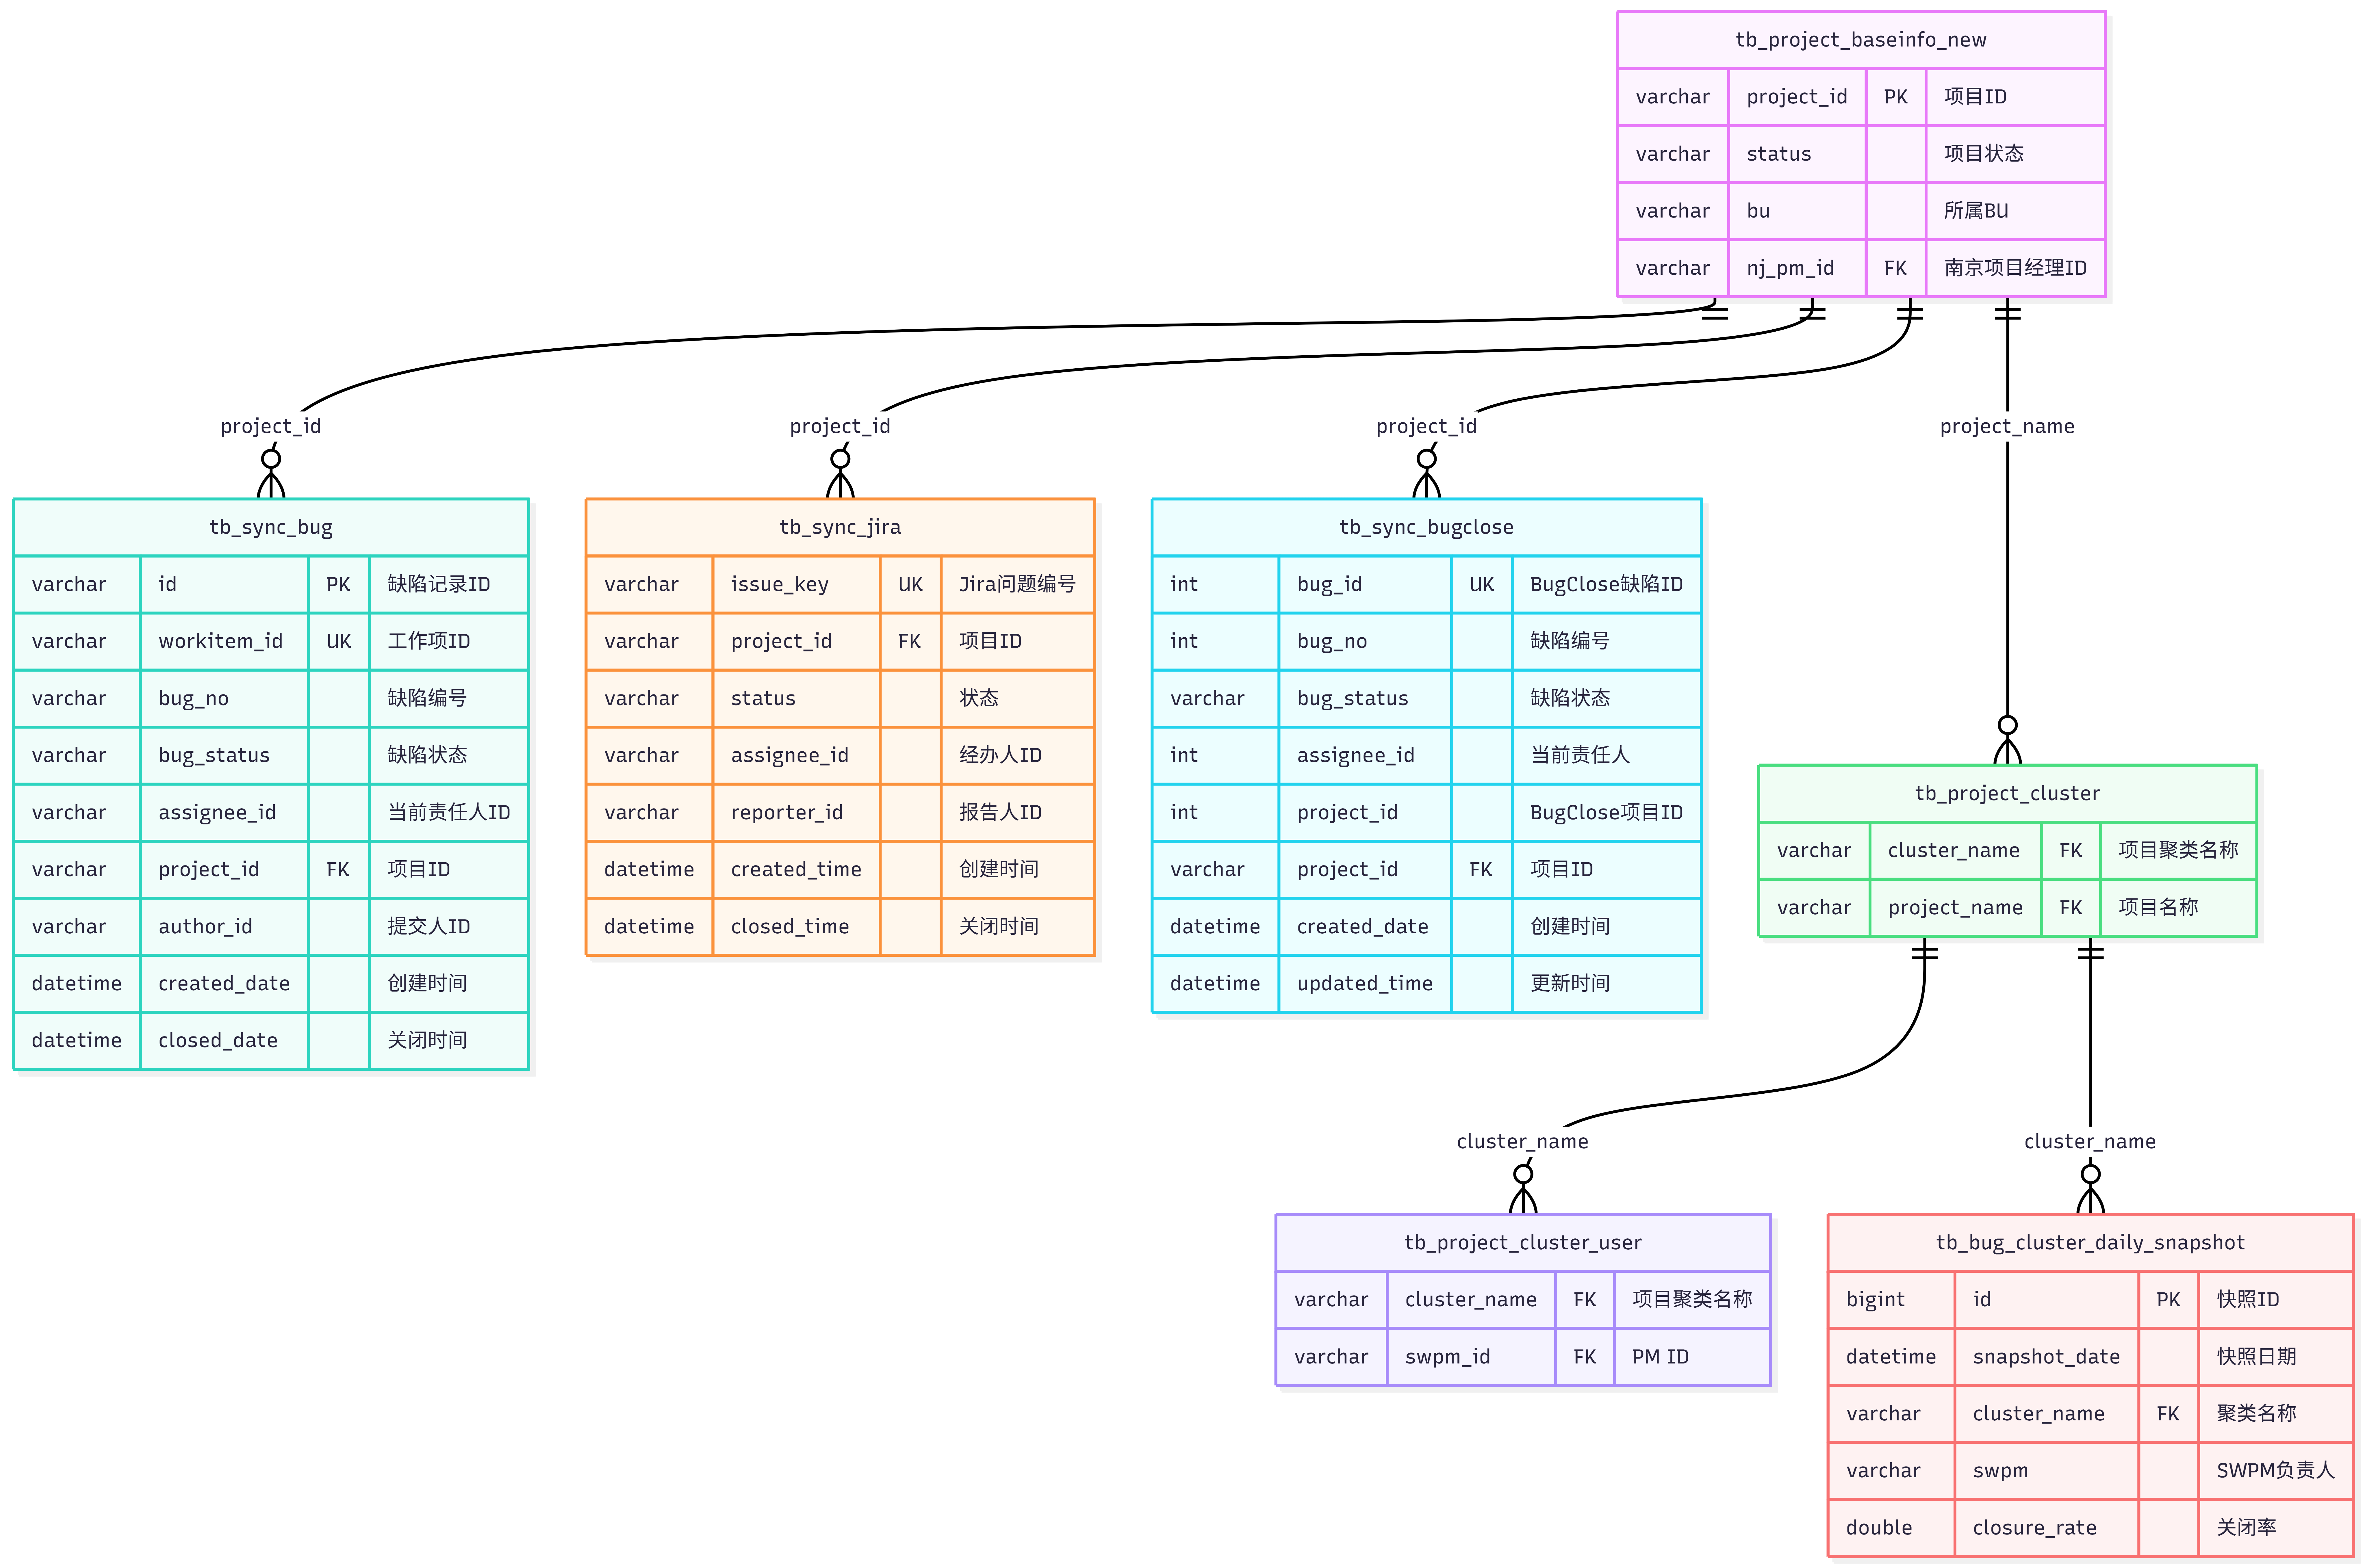
\includegraphics[width=0.7\linewidth]{imgs/ER图-缺陷聚类.png}
		\caption{缺陷聚类E-R图}
		\label{fig:er-bug-cluster}
	\end{figure}
	
	在该模型中，\verb|tb_project_baseinfo_new| 仍然作为项目主数据表，用于提供项目编号、项目状态、所属 BU 和项目负责人等基础信息。\verb|tb_sync_bug| 用于保存从 Trinity 系统同步的缺陷数据，包括缺陷记录 ID、工作项 ID、缺陷编号、缺陷状态、责任人、所属项目、创建时间和关闭时间等字段。\verb|tb_sync_jira| 用于保存从 Jira 系统同步的问题数据，包括 Jira 问题编号、问题状态、经办人、报告人、创建时间和关闭时间等信息。\verb|tb_sync_bugclose| 用于保存从 BugClose 系统同步的缺陷数据，包括 BugClose 缺陷 ID、缺陷编号、缺陷状态、责任人、所属项目和更新时间等字段。三类缺陷表均通过项目编号或项目名称与项目基础信息表建立逻辑关联。
	
	此外，系统使用 \verb|tb_project_cluster| 表维护项目与项目聚类之间的对应关系，使用 \verb|tb_project_cluster_user| 表维护项目聚类与 SWPM 负责人之间的对应关系，使用 \verb|tb_bug_cluster_daily_snapshot| 表保存项目聚类每日缺陷快照。通过这些表，系统可以按项目群或项目聚类维度统计未关闭缺陷数量、新增缺陷数量、关闭缺陷数量和关闭率等指标。该设计能够满足管理人员从单项目维度和项目群维度分析质量风险的需求。
	
	\item 重大问题管理模块用于记录项目研发和交付过程中出现的关键质量问题、交付风险和客户关注问题，其 E-R 模型如图\ref{fig:er-serious-problem}所示。
	
	\begin{figure}[htbp]
		\centering
		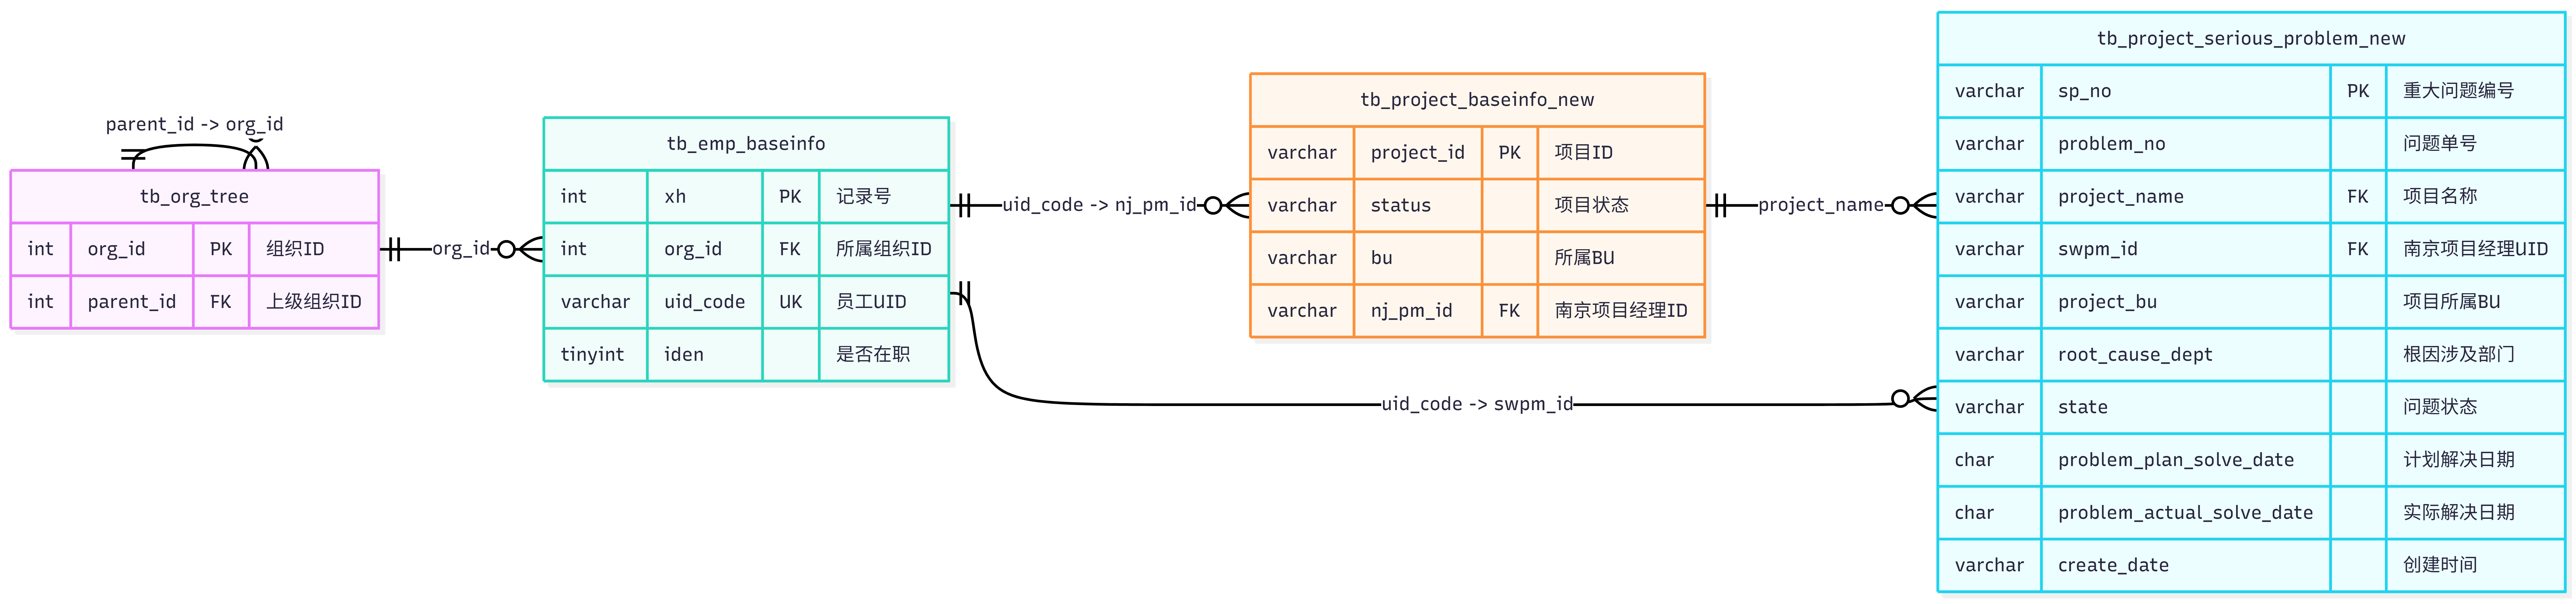
\includegraphics[width=0.7\linewidth]{imgs/ER图-重大问题.png}
		\caption{重大问题E-R图}
		\label{fig:er-serious-problem}
	\end{figure}
	
	该模型中，\verb|tb_project_serious_problem_new| 是重大问题管理的核心实体，用于保存重大问题编号、问题单号、项目名称、南京项目经理 UID、项目所属 BU、根因涉及部门、问题状态、计划解决日期、实际解决日期和创建时间等信息。项目基础信息表 \verb|tb_project_baseinfo_new| 通过项目名称与重大问题表建立逻辑关联，用于说明重大问题所属项目。员工基础信息表 \verb|tb_emp_baseinfo| 通过 \verb|uid_code| 与重大问题表中的 \verb|swpm_id| 建立逻辑关联，用于标识重大问题对应的南京项目经理。员工表又通过 \verb|org_id| 与组织表 \verb|tb_org_tree| 关联，从而可以进一步追溯问题涉及人员所属组织。
	
	通过该 E-R 模型，系统能够支持重大问题分页查询、新增、编辑、详情查看、状态跟踪和数据导出等功能。重大问题表不仅记录问题本身，还记录问题所属项目、责任人、根因部门和计划解决时间等关键管理信息，因此能够为项目复盘、质量改进和管理层决策提供数据依据。
	
\end{enumerate}
整体来看，四组E-R图分别从工时、项目、缺陷和重大问题四个维度，把系统的核心数据实体及其关联关系固定下来。建模过程遵循数据库设计总体原则。后续各功能模块的详细设计，均围绕本节E-R模型展开。

\section{本章小结}
本章重点论述了系统核心业务模块的详细设计，介绍了各个功能模块有关的类和接口以及关联关系，同时详细展示了几个关键点的具体设计和优化，给出了数据库中相关表结构的设计。下一章节，将基于系统的详细设计方案，展开对系统实现与测试的介绍。